\documentclass{newrucsthesis}
\setlength{\parindent}{0in}
%\usepackage{fullpage}
\usepackage[english]{babel}
	\addto{\captionsenglish}{\renewcommand{\bibname}{References}}
\usepackage[utf8]{inputenc}
\usepackage{graphicx}
\usepackage{mathtools}
\usepackage{setspace}
\usepackage{courier}
\usepackage{enumerate}
\usepackage{fancyhdr}
\usepackage{lastpage}
\usepackage [autostyle, english = american]{csquotes}
\usepackage{url}
\usepackage{float}

% ====================================================================== %
% test listing system
\usepackage{listings}
\usepackage{color}


\definecolor{codegreen}{rgb}{0,0.6,0}
\definecolor{codegray}{rgb}{0.5,0.5,0.5}
\definecolor{codepurple}{rgb}{0.58,0,0.82}
\definecolor{backcolour}{rgb}{0.95,0.95,0.92}

\lstdefinestyle{mystyle}{
    backgroundcolor=\color{backcolour},   
    commentstyle=\color{codegreen},
    keywordstyle=\color{blue},
    numberstyle=\tiny\color{codegray},
    stringstyle=\color{yellow},
    basicstyle=\footnotesize,
    breakatwhitespace=false,         
    breaklines=true,                 
    captionpos=b,                    
    keepspaces=true,                 
    numbers=left,                    
    numbersep=5pt,                  
    showspaces=false,                
    showstringspaces=false,
    showtabs=false,                  
    tabsize=4
}

\lstset{style=mystyle}
% ====================================================================== %

\everymath{\displaystyle}
\graphicspath{ {images/} }
\restylefloat{figure}

\begin{document}

	\pagenumbering{roman}
	\onehalfspacing
	\begin{titlepage}
    \begin{center}
        \vspace*{1cm}
        
		\Huge
        \textbf{Towards a Facial Recognition Workstation}
        
        \vspace{0.5cm}
		\LARGE
        With Accompanying Examples
        
        \vspace{1.5cm}
        
        \textbf{Matthew Shane Kingon} \\
        \textbf{Supervisor: Prof EP Wentworth}
		
        \vfill
        
		Submitted in partial fulfilment of the \\
		requirements for the degree of BACHELOR OF \\
		SCIENCE (HONOURS) of Rhodes University
        
        \vspace{0.8cm}
        
        
\includegraphics[width=0.4\textwidth]{Crest.png}
        
		\Large
        Computer Science Department\\
        Rhodes University\\
        Grahamstown, South Africa\\
		\date{April 27, 2015 -- \today}
        
    \end{center}
\end{titlepage}

	% =================== =================== %
	% Preliminaries to be Numbered with 
	% roman numerals
	% =================== =================== %	
	\section*{Abstract}
		This work looks into the feasibility of using facial recognition to track lecture/classroom 
		attendance.  It is clear that any such system would need to take into account many normalization 
		concerns, to this end, this work employs a facial recognition workstation to easily test such 
		techniques.  A literature study points to an illumination correction algorithm, known as the Mean
		Illumination Estimation.  Results correlate strongly with the literatures claims that such a method 
		would best the current standard for illumination correction.  However, for our specific classroom 
		environment	we conclude that such a method is not adequate.  This work also looks into applying a 
		minimum cost assignment optimisation upon the output provided by the Eigenface Algorithm.
	
		\newpage
	
	\section*{ACM Classification}
		\begin{enumerate}
			\item Computing methodologies---Artificial intelligence---Computer vision---Computer vision problems---Object recognition;500
			\item Computing methodologies---Artificial intelligence---Computer vision---Computer vision tasks---Biometrics;500
			\item Mathematics of computing---Mathematical analysis---Numerical analysis---Computations on matrices;500
			\item Computing methodologies---Symbolic and algebraic manipulation---Symbolic and algebraic algorithms---Optimization algorithms;300
			\item Applied computing---Physical sciences and engineering---Mathematics and statistics;100
		\end{enumerate}
		Other Keywords:
		\begin{itemize}	
			\item Facial recognition workstation;500
			\item Illumination normalization;500
			\item Multiple cost assignment minimization;300
			\item Hungarian Algorithm;300
		\end{itemize}
		\newpage
	
	\section*{Acknowledgements}
	I would like to acknowledge the financial and technical support of 
	Telkom SA, Tellabs, Easttel, Bright Ideas 39, THRIP and 
	NRF SA (UID 75107) through the Telkom Centre of Excellence in the
	Department of Computer Science at Rhodes University. \\
	
	I would like to acknowledge The Rhodes University Computer Science 
	Honours class (2015) for minor latex usage technical support over 
	the past year.
	\newpage	
	
	\tableofcontents
	\newpage	
	\listoffigures
	
	\newpage

	% =================== =================== %
	% Main body of work separated out into 
	% separate files to be Numbered with 
	% arabic numerals
	% =================== =================== %
	\newpage
	\pagenumbering{arabic}
	
	% introductory chapter explaining what my 
	% project is all about;
	% Motivation for the research – why and put in perspective
	% Nature of research = research questions to be addressed
	% + key concepts + hypothesis
	
	% Brief description of approach – preface to Methodology
	% section later. Broad but clear view.
	% Organization of rest of thesis
	\chapter{Introduction}
	\section{Project Background}
	\subsection{Background context}
		Despite modern day technology many school environments still struggle with the problem of class/lecture 
		attendance tracking.  Some may ask, why do we need to track attendance?  Tracking attendance 
		has many useful benefits for schools and universities the obvious one is that many students try skip 
		lectures to avoid work.  Thus tracking their attendance would help in identifying such students.  This 
		would, hopefully, result in greater attendance of such classes/lectures. \\

		The existing solution to this problem has varied slightly but for the most part has either been a simple 
		piece of paper passed around the class letting the students sign/tick their names off (mostly used in 
		universities), or a roll call at the start of the class by teachers in lower level class room environments 
		(primary/high-school).  \\

		Thus it shouldn't come as a surprise that there have been many attempts to solve the problem of lecture 
		attendance tracking and hence remove some issues.  Some of the main ideas put forward are: barcode scanners
		~\cite{barcode}, RFID systems~\cite{RFID} and the ever popular fingerprint scanners~\cite{fingerprintsystems}.  
		The problem with these systems is that they are still all rather intrusive workarounds, requiring students to 
		take an active part in their attendance tracking, this results in either lines outside of lecture room venues 
		as students wait to verify that they are in attendance, or alternatively, a rather distracting procedure to do 
		while they could be listening to the lecture. \\

		Past papers on this topic have addressed the existence of these issues in some context or another
		~\cite{PatelDoaSAMSURaFR,BalcohAfEAM,KarheSASAUFR}.  Now as many have recognized that facial recognition has 
		the potential to be a very simple, and non-intrusive means of tracking attendance, as in the ideal case it
		would simply need a camera at the front of the class and as the lecture goes on it identifies all students 
		present.  However, the technology available today is still not robust enough, hence the need for further 
		research, development and refinement in this field.  \\
		
		Some points of interest to consider are lighting, as it is a very big problem that has had many attempts at a 
		solution most are not satisfactory as they degrade the image too extensively.  The required camera quality is 
		also an area of interest.  Ideally it would be good to get a solution that can work with an off-the-shelf 
		web-cam.  \\		
		
		It should be noted that facial recognition isn't a perfect science to start with.  Many solutions don't even 
		take into account that they are attempting to recognize a face.  These algorithms could be more accurately
		described as object recognizers, some rather popular examples of this type of system include Egienfaces, 
		Fisherfaces. This work takes into account many of these issues and also attempts to use environment specific 
		knowledge to recognize students (the fact that we know both the training set and class set). \\
		
		As stated there have already been numerous attempts at a solution for classroom attendance.  Some have been 
		more successful than others.  However, this work differs from the others as we hope to design a system that 
		can be easily extended or modified to test out new ideas to improve recognition.  Not only do we wish to offer 
		a system one can easily plug new normalization techniques into, but also able to make use of additional 
		information that pertains to a specific problem a user may be facing. \\
		
		Possible additional information that could be exploited include the knowledge that students tend to sit in the 
		same area each day often varying their position by little more than a seat or two.  This knowledge could be used 
		to strengthen accuracy ratings should an individual known to sit at that location is identified.  Another aspect 
		could be useful to such a system is the knowledge that prior to lectures it is already known who should be there.  
		Thus an attempt can be made to optimize the solution between two sets, namely a set of present faces, and the 
		class-list set. \\

		Facial recognition is a complex field and has been well researched over the past decades even so, it is far from 
		being a fully understood or solved problem.  An aspect clearly portrayed by the fact that there are many 
		variations in methods and techniques out there to solve this problem. \\
		
		The work provides an illustrated application of this platform by implementing facial recognition for lecture 
		attendance tracking.  This work focuses on extending the pre-processing side of the tool-kit using the already 
		provided OpenCV implementation of Eigenfaces to do the actual recognition.  One notable addition would be adding 
		the Mean Illumination Estimation algorithm.   Some more concepts that are added include; image cropping, 
		orientation correction and plane alteration.  All of the above concepts describe various aspects of image 
		normalization.
		
	\subsection{Making a Toolbox}
		A constantly developing key aspect of this research project is creating a facial recognition tool-kit.  
		This platform will act as scaffolding for the addition of any features related to facial recognition, be it 
		pre-processing or actual facial recognition algorithms.  The idea is to selectively add relevant image 
		manipulation techniques or other such features to the code base, thus allowing the client to mix and match 
		them and after application get a report stating how successful the combinations that where chosen are.  Some features 
		would be cropping the faces out from the background noise, others would aim to control lighting.   \\
			
			
\section{The Project}
	\subsection{Description of this Work}
		The overall goal of this research is to determine if it is possible to efficiently automate attendance tracking 
		in lectures via facial recognition.  In a related project (not directly part of this work) a video stream of the 
		class is analysed to extract and cluster faces of the same individual.  In this work we take a direct approach that 
		finds the best match for each normalized cluster in the class list of faces.  A second approach is theorised that 
		would simultaneously take into account all possible matchings and find a globally optimized assignment of each 
		cluster to the class list. A comparison of matching accuracies for the two techniques could then be provided to 
		determine the benefits or trade-offs.

	\subsection{What my code should do} 
		My code should be able to: take input of the form of a folder of images.  In each image would be a single face 
		with around ten such images~\cite{OpenCVTut} per subject.  I would then take those images, put them through some form of 
		normalization, thereafter put them through the recognizer which will then compare the created feature vector 
		against those created from the database which was used to train the system.  Doing this comparison, the system 
		would determine the most likely candidate for the subject in question.  

	\subsection{Language choice}
		The language my code will be implemented in will be Python, on a windows based OS, making use of the OpenCV image 
		processing library.  The reason I've chosen Python is for its ease of use with regards to image processing and 
		the intention of this work is that of a working proof of concept so efficiency is not a concern at this stage.  
		I made the choice of using OpenCV as it is the most robust open source library package for image processing.  
		Another factor in favour of OpenCV is that it is open source and thus free.  Part of the aim of this work is to 
		create a low cost system. 
		
	\subsection{Things to note}
		As with most academic work, some formality of raw data is often required, for this work this data is facial images or more 
		accurately, databases of facial images.  I would need such databases to train my system to recognise faces in a 
		controlled manner.  Once I have refined my system to recognise these faces with a satisfactory degree of accuracy 
		that conform with other literature, I will extend it to recognize faces in every day images.  Ultimately this work will be testing using 
		data obtained from a lecture venue environment. \\

		Luckily there is a ready supply of such collections.  A starting point to find such databases would be the site
		~\cite{urldatabases} which catalogues, with descriptions, many such databases.  An initial overview of the site 
		indicates that I should look into the Yale B face Database as it contains far more variety than others especially 
		when it comes to illumination changes.  However, the FERET database makes use of notably more consistent backgrounds.  \\
		
		Another database I will look at is the AT\&T database~\cite{ATTDATA}.  It is smaller than the Yale B database, but has more realistic real 
		world orientations of faces and the more likely accurate representation of images captured in a classroom environment.
	
\section{Other Key Aspects}
	\subsection{Computer Vision}
		For my project I need to know how to recognise faces, hence a useful starting point would be how to interpret images.  
		Both these requirements fall under computer vision.  Computer vision is the field focusing on using image processing 
		to gain information from images for a computer to use.  Ideally this would let the computer view the world in much 
		the same manner as how we humans see it. \\
		
		Computer vision makes use of edge detection, object recognition, feature detection and many other techniques to help 
		make a computer see the world as we do.  This concept is an infinitely harder task than someone outside the field of 
		computer vision may believe.  Mostly due to the effortlessness at which a human brain seems to interpret what it is seeing.
		~\cite{szeliski2010computer}.  More specifically this work will need to understand the interpretation of an image in 
		the Numpy/OpenCV environment.
		
	\subsection{Illumination Normalization}
		Apart from my main aim to verify Faces in images there are certain other considerations to note.  Before I can start 
		to verify faces in images I would need to normalize those images.  Normalizing with respect to image processing is the 
		act of taking images of varying lighting, orientation and alignment and converting them into a semi-consistent form
		~\cite{FDGFN2009}.  \\
		
		Not only will I need to normalise a face but also combine clusters of faces, either finding the best face to use or 
		normalize each face cluster into a single image in an attempt to create an \emph{Average face} for an individual.  
		Another method of using multiple images is to individually normalize and score them all and see whom the majority 
		are classified as.
		
	\subsection{Global/Greedy Optimisation}
		This work made use of OpenCV's eigenface algorithm which makes use of a greedy best pick algorithm.  Such a greedy 
		technique takes a probe face, scores it against all training data and reports on the best match it got, less accurate 
		than other methods but fast. \\
		
		In this work it would be an interesting idea to compare greedy and global based optimising techniques.  A global technique 
		would try find the best fitting of faces such that we have the lowest possible scores linking each face~\cite{GlOP1989}.  
		This would imply we would achieve higher accuracy but possibly a more computationally expensive system.  \\
		
		Clearly a classroom environment where we have a set class-list and know that we should have those students present lends 
		itself nicely to a global optimisation scoring system.  Comparing them would highlight if performing such an optimisation
		provides clear benefits over the in-built greedy match in terms of accuracy at the cost of complexity to implement and 
		computation time. \\
		
		This work explores a global match optimisation idea in chapter four,  but we were not able to implement such a system due to constraints 
		that will be discussed later.
	
	% Chapter containing reviews of all my source 
	% material expanded upon in the rest o the 
	% thesis
	\chapter{Research of Background Literature}
	\section{Introduction to Literature Review}
	\subsection{Readings for Literature Survey}
		This section will highlight some sources I have found that will most likely be of aid to my project; To start off; I 
		will need some form of text that can explain in detail the process of facial verification as well as image processing 
		concepts in general. To this end, I have highlighted ~\cite{szeliski2010computer} as one potential, probably invaluable, 
		source.  Another useful resource would be ~\cite{bradskeiLOCVwtOL} to provide a general overview to the usage of OpenCV. \\
		
		In order to run facial verification on a collection of images it would be wise to know how best to align the faces on 
		those images.  This is a process that falls under the aspect of normalization.  To help me figure out how this works I 
		have highlighted ~\cite{hasan2011improving} as possible useful information. \\
		
		Another aspect of normalization would be illumination normalization as stated I will be looking in-depth into the MIE 
		algorithm as proposed in~\cite{LuoaRINMBoMEfFR}.  \\
		
		Another area I would need to become proficient in would be mathematical optimization.  Namely, global optimization 
		techniques.  To help me with this I have highlighted ~\cite{Hungarian_alg}	as a possible method. \\
		
	\section{Overview of Used Systems}
		The toolbox is developed using Python and the OpenCV library in conjunction with the mathematical, 
		Numpy library.  However, too limit the scope of the project from getting too ambitious the system this 
		work implements will, at least initially, be console based. \\
		
		% OpenCV
		OpenCV is one of the most popular image processing libraries.  It was released under a BSD license 
		and thus is free for both academic and commercial use.  The provided functionality is highly optimised, 
		having been designed primarily for real-time computer vision.  The code base used to implement the 
		library functions is C/C++ to provide the most optimised solutions~\cite{OpenCVorg}.  \\
		
		% Python
		Python is an open source programming language designed for ease of use and learning.  It is an open 
		source project, hence free for use in any project you could need it for.  It is designed to interface 
		well with various aspects in computer science e.g. databases, web-servers, even other coding languages 
		with a relatively easy to use wrapping system to add in functionality provided in non-python libraries 
		for example the  afore mentioned OpenCV image processing library~\cite{Pythonorg}. \\
		
		\newpage
		% Numpy
		Numpy is a mathematical library focusing around matrix manipulations employing a powerful N-dimensional 
		array object.  It provides functionality to integrate C/C++ or Fortran code.  As with OpenCV it is licensed 
		under the BSD license and hence free for public or commercial use.  It is one of the prerequisites of OpenCV 
		in Python primarily because of its powerful matrix data representation, hence a good solution for a machine 
		representation of an image.  It permits its matrices to contain arbitrary data-types allowing ease and speed 
		of use in most database systems~\cite{Numpyorg}.
	
	\section{Image representation overview}
		The OpenCV library was chosen as it provides many useful image manipulation and computer vision techniques.  
		However, this means a solid understanding of how OpenCV represents these images is required to best make use 
		of the provided functionality.  \\
		
		OpenCV has already overloaded many mathematical operations to take their representation into account.  Hence 
		it is possible to simply take two images imported via ``cv.imread(...)'' or other such methods and add or 
		subtract them with a (``+'' or ``-'').  However, this is implemented only for basic mathematical operations.  When
		one wishes to perform more complex arithmetic procedures one needs to take into account the representation of 
		an image. \\
	
		The matrix representation that describes the images this work makes use of is that of a 
		simple 2D array or, mathematically, a 2D matrix.  This comprises the core of an image class.  However, there 
		are many other headers that are provided by an image class, these include headers that describe the width and 
		height of the image, the mathematical representation of the values inside the matrix (i.e. 8,16,32 bit numbers 
		weather or not they are floats etc), name of the image, how many channels it has i.e. (Red, Blue, Green) and whether 
		or not it has an alpha channel (transparency).  These comprise the most important features of an image
		~\cite{bradskeiLOCVwtOL}.\\
		
		\newpage
		It is noted that OpenCV makes use of Numpy, a mathematical matrix library, for many of its built-in procedures.  
		This is possible as OpenCV interprets the way Numpy represents matrices as images.  Thus is useful to client
		programs as Numpy can thus be used to take care of the heavy lifting with regards to manipulating an image's pixel 
		data.  This provides the client with a simple view of an image as a 2d array that can be manipulated as such.
		
		
		\section{Eigenface Algorithm}
			\subsection{Intuitive description}
			One of the most popular object recognition algorithms makes use of the mathematical eigenvector/principle 
			analysis for component analysis PCA is already implemented in OpenCV specifically for faces and is called 
			the Eigenface method. \\
			
			The Eigenface method of facial recognition works by taking the high dimensional face images represented 
			mathematically as an $m \times n$ matrix.  Providing it with N such images it takes them and finds the 
			average of the matrices(images) i.e. sum them together pixel by pixel and divide by N.  With this ``Average 
			face'' new images are created by subtracting the training images from the average image.  This represents each 
			face as a difference, or deviation from the average.  Once this has been done a set of orthonormal basis 
			matrices are calculated.  Each difference face can then be projected onto the bases, resulting in a feature
			vector of co-efficients which best represent these ``difference faces''.  Indeed, once a system is trained with 
			a set of images, given any of these training images one should be able to get coefficients that reconstruct 
			the original face exactly.  The reconstruction is done by adding the average face plus a linear combination 
			of the basis matrices.  The feature vector obtained determines the weighting of each basis matrix to enable 
			complete reconstruction of the training face. \\ 

			With these we can construct a face that somewhat represents one of the individuals we used in our training 
			set by taking the average face and adding varying components, determined by	a set of coefficients, of our 
			basis images.  This set of coefficients is called the feature vector of the difference face providing us the 
			means of recognition, as for similar faces (presumably of the same person) the feature vectors will be very 
			close.  
		
			\subsection{Training}
			The Eigenface method requires training, this means that it needs to be given images 
			of the faces it should recognize.  For example the set of faces shown in figure ~\ref{fig:Face_set}:
			
			\begin{figure}[h!]
				\centering
				\caption{Example of a training set.  Some faces are blacked out due to lack of permission.\label{fig:Face_set}}
				\includegraphics[width=105mm,height=105mm]{training_set_permitted.png}
			\end{figure}
			
			It then takes each image and converts it into a high dimensional vector created as: 
			
			\[ 		\Gamma_n = (Width)\times(Height) \quad | \quad n = 1,..,N \]
			
			Where N is the number of training images you have.	the result is a set {S} of N such face 
			image matrices: 			
			
			\[		S = {\Gamma_1,\Gamma_2,\Gamma_3,...,\Gamma_N} 		\]	
			
			After this is done the method finds the average face given as:											
			
			\[		\varphi = \frac{1}{N} \sum_{n=1}^{N} \Gamma_n  			\] 
			
			The average face constructed from this training set can be seen shown below in Figure ~\ref{fig:Ave_face}:
			
			\begin{figure}[h!]
				\centering
				\caption{The Average Face\label{fig:Ave_face}}
				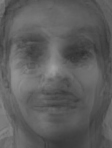
\includegraphics[width=200px,height=270px]{mean_image.png}
			\end{figure}
			
			Once the ``average face'' is determined the method calculates the difference $\phi$ between it and 
			each image in the training set.

			\[ 		\phi_n	=  \Gamma_n - \varphi						\]  
			
		
			We next obtain the covariance matrix C which we need for its Eigenvectors/values ($v_{n}, \lambda_{n}$) 
			respectfully. We obtain C via:
			
			\[		C 	= \frac{1}{N} \sum_{n=1}^{N} \phi_n \phi_n^T 	\] 	
			\[			= AA^T											\]

			where:
			\[ 		A = {\phi_1 , \phi_2, \phi_3, ... , \phi_n} 		\]

			\emph{Note, the superscript T implies the corresponding matrix/vector is transposed.}			
			
			The core concept of Eigenvector/value pairs is that given a matrix operation (in our case C) 
			on a vector ($v_{n}$) then this is equivalent to some scalar ($\lambda_{n}$) multiplied by that same vector. 
			
			\[		C v_{n} = \lambda_{n} v_{n} \quad n = 1,2...,N 		\]
			
			This relation allows us to find $v_{n}$ and $\lambda_{n}$ of C.  We create a new matrix $\omega$ by 
			combining these eigenvectors ($v_{n}$) ordered in descending eigenvalues ($\lambda_{n}$).  
			We then use this new construct to determine our feature vectors for each training face. via:			
			
			\[		y_n = \omega^T(\phi_n) 	\quad 	n = 1,2...,N 		\]
			
			Where $\phi_{n}$ as seen above is the difference image between the training image $n$ and the average image $\varphi$
			Note: although $\phi$ represents an image, mathematically we are viewing it as a single line vector.  We multiply this 
			vector by our created matrix $\omega$ to yield the feature vectors $y_n$ for our training data.  Thereafter we compare 
			any future image against these vectors to determine who they best match against.
			
		
			\subsection{Prediction}
			Once the recognizer has been trained with the input training data, what it stores are the average face, orthonormal basis 
			matrices and the feature vectors for each individual in the training data.  Then it can be fed some unseen images of the
			people it has trained on and see how it fares.  Herein we describe the procedure of taking a new image and testing it against 
			our trained recognizer. \\  
			
			To transform a new face into its Eigenface components.  First, subtract our input image $\Gamma$ from our mean image 
			$\varphi$ then multiply by the eigenvector matrix $\omega$.  Doing so, we produce the feature vector $x$:		
			
			\[		x = \omega^T(\Gamma - \varphi) \]
			
			We now determine which of the training faces is the best fit by finding the feature vector of the training face $y_n$ with the 
			minimum euclidean distance to the feature vector of the probe face $x$ we do so by calculating all these differences $\varepsilon_n$:
			
			\[			\varepsilon_n = \| x - y_n \|	\] 
			
			Then take:
			\[			min(\varepsilon_n)	\]
			
			To get the best match to our training data.  This distance also offers a means of indicating the confidence of this match. \\
			
			It should be added that Euclidean distance is not the only means of determining how different vectors are.  Indeed, for our 
			purposes it is possible that it could even be detrimental to the recognition rates.  Another solution would be to use the 
			absolute distance.  This is still not 100\% ideal but it may not have as much of an effect on our accuracy scores. \\
			
			If $\varepsilon_n$ is below a certain threshold defined within the algorithm the face is 
			considered to be known and represented by $\Omega_n$.  If instead the  $\varepsilon_n$ is 
			above the threshold the image is determined not to be face from the training data or indeed 
			a face at all.  If the threshold value is chosen too small only very close approximations 
			to our training set will be accepted by the algorithm leading to a higher accuracy, at the 
			other end, if the threshold is too large the algorithm will generate many false positives.  
			If the image is a face you know belongs to one of your subjects but the system determines it 
			is an unknown, then you could subsequently identify the individual by other means and then choose 
			to add it into the set of known faces and repeat the training steps i.e. incorporate the latest 
			image of the individual into the system (Doing so may be appropriate under certain circumstances 
			eg. the subject gets a hair cut, shaves his beard etc).
			
			\subsection{Summary of EigenFaces}
			So in summary, the Eigenface algorithm is provided with a set of face images to train on, then 
			once it is trained it is given an image, presumably a face of one of the people from the training 
			set, it will then ideally match it to the correct person and report how close the two feature 
			vectors are to each other are in the space provided.  \\
			
			It is important to note even though this method is called the Eigenface method, nothing about 
			it forces the use of facial images, indeed it is simply a image recognizer that has been shown 
			to work well on faces.  An example of PCA systems being used on non-face objects can be seen in
			~\cite{plantClassification} where they use the idea to identify different plant types based on 
			individual leaves from each plant.  One known weakness is that lighting will have a very large 
			impact on its performance, as opposed to other methods.  Though in other methods lighting does 
			play a part and is something you wish to remove, it is highly detrimental to the Eigenface method. 
			Thus to build a robust system lighting will need to be normalized and compensated for. \\
		
			The above mathematical understanding of the implementation of the Eigenface algorithm was 
			achieved via the tutorial found at~\cite{urlEgienFaceTut}.  Matthew Turk and Alex Pentland 
			developed the original algorithm~\cite{turk1991eigenfaces}.

	\section{Normalization}
		\subsection{Cropping}
		As has been stated the Eigenface algorithm is an image recognizer, thus background image 
		data will have a drastic impact on its performance and recognition rates.  For this reason 
		it is important to get rid of as much of an images background as possible.  
		Cropping an image is easy by hand, but the point of this whole exercise is to automate 
		the process of facial recognition as much as possible.  Hence, to crop a face out 
		of an image the face would first need to be found.  To this end, we would need a face 
		identifier. \\
		
		This work already implements such a feature in a separate component of the project ~\cite{MarceloFIFLA}.  
		As this work attempts to create a facial recognition tool-kit, the client can specify the bounds 
		of the cropping procedure once the face is found giving said user the ability to crop it 
		aggressively or not at all. \\
		
		Preliminary testing does indeed show that cropping an image has an effect on the recognition 
		rate.  However, these have been manual crops that do not resize the image nicely.  Also, some 
		faces are simply not well cropped with a lot of background left in the image.  Another improvement 
		that can be attempted is to white/black out the remaining background so that for all images the 
		background makes the same contribution to the algorithm's scoring system. 
		
		\subsection{Lighting}
		Lighting plays a very integral role for the Eigenface algorithm.  As such, we expand upon this concept
		more fully in chapter 3 by providing a strong background as to why lighting is an issue and experimenting 
		with various ways to overcome said issues posed by illumination. 
		
		\subsection{Alignment and scaling}
		The final big normalization issue would be face alignment and scaling, when a photo is taken/camera is 
		run, the faces wont be all similarly scaled or aligned.  This is something the system needs to take
		into account. \\
		
		Hence this becomes a software problem.  Most alignment algorithms find suitable features in a face with 
		which to re-align the face correctly~\cite{hasan2011improving}.  Such features can include the location 
		of the eyes in a face and use these to re-align the head so that it is as straight on as possible.  This 
		could be achieved by taking the eyes, drawing a line between them and levelling this line out so that it 
		is straight.  It should be noted that the nose can also be used as an alignment feature but the eyes are 
		favoured as they provide a longer axis to align with.  \\
		
		Scaling of a face can also be achieved through the distance between the eyes.  The image as a whole 
		can be scaled bigger or smaller so that this distance conforms to a fixed value. 	
		
\section{Summary}
	This work aims to create a facial detection and recognition tool-kit.  However, the true extent of this goal 
	is beyond the scope of this paper.  The main goal of this work, at least initially, is to get an end-to-end 
	system up and running even if many features require manual input.  For example; cropping and alignment can be 
	done by hand by prompting the client to locate the centre of the eyes in an image.  Taking these locations, it
	can realign the head and set the eyes to fixed locations. \\
	
	The bulk of the current work focusses on the Eigenface algorithm for facial recognition.  More importantly, 
	it attempts to fully understand and implement the normalization technique called the Mean Illumination 
	Estimation~\cite{LuoaRINMBoMEfFR} and ascertain the benefit on Eigenfaces accuracy rating by using this 
	pre-processing technique. \\
	
	As was explained earlier a key aspect of the system is that its framework and structure will be easy to extend 
	and utilise.  Providing future researchers with the ability to add the functionality they desire whether they 
	wish to add extra pre-processing methodologies or a more robust recognition algorithm.
	
	% Chapter to lay out the theoretical design 
	% my project will conform to.
	\chapter{Illumination}
	\section{The Issue of Illumination}
Lighting plays a very big role in all facial recognition, identification or just about any image processing problem.  
To the human eye, it can be an almost undetectable irregularity in the world we observe but to a computer that must 
inspect each and every pixel within an image to determine what it is observing, even the slightest change in lighting 
make each pixel value change dramatically.  This problem can complicate any image processing techniques. \\

To better appreciate the problem it should be noted that there are an abundance of illusionary images that manage to 
fool the human brain.  These examples are often very specifically designed for this very purpose. However, it does
illustrate the point.  The example shown in fig:[~\ref{fig:OIE}] may be an old one, but will still often fool most people 
you show it to; the two blocks with the orange dot are in fact, the same shade of grey, the two orange dots are also 
the same colour.  Some may see it right away but even so it takes effort to see it.  This is due to the fact that your 
brain logically assumes that the lower dot is on top of the brighter block set and hence should be brighter than the 
darker block set around it which it is.  However, it is not brighter than all dark blocks in the image, this occurs 
because your brain doesn't take into account the shadow cast upon the blocks.	

	\begin{figure}[H]
		\centering
		\caption{Optical Illusion example\label{fig:OIE}}
		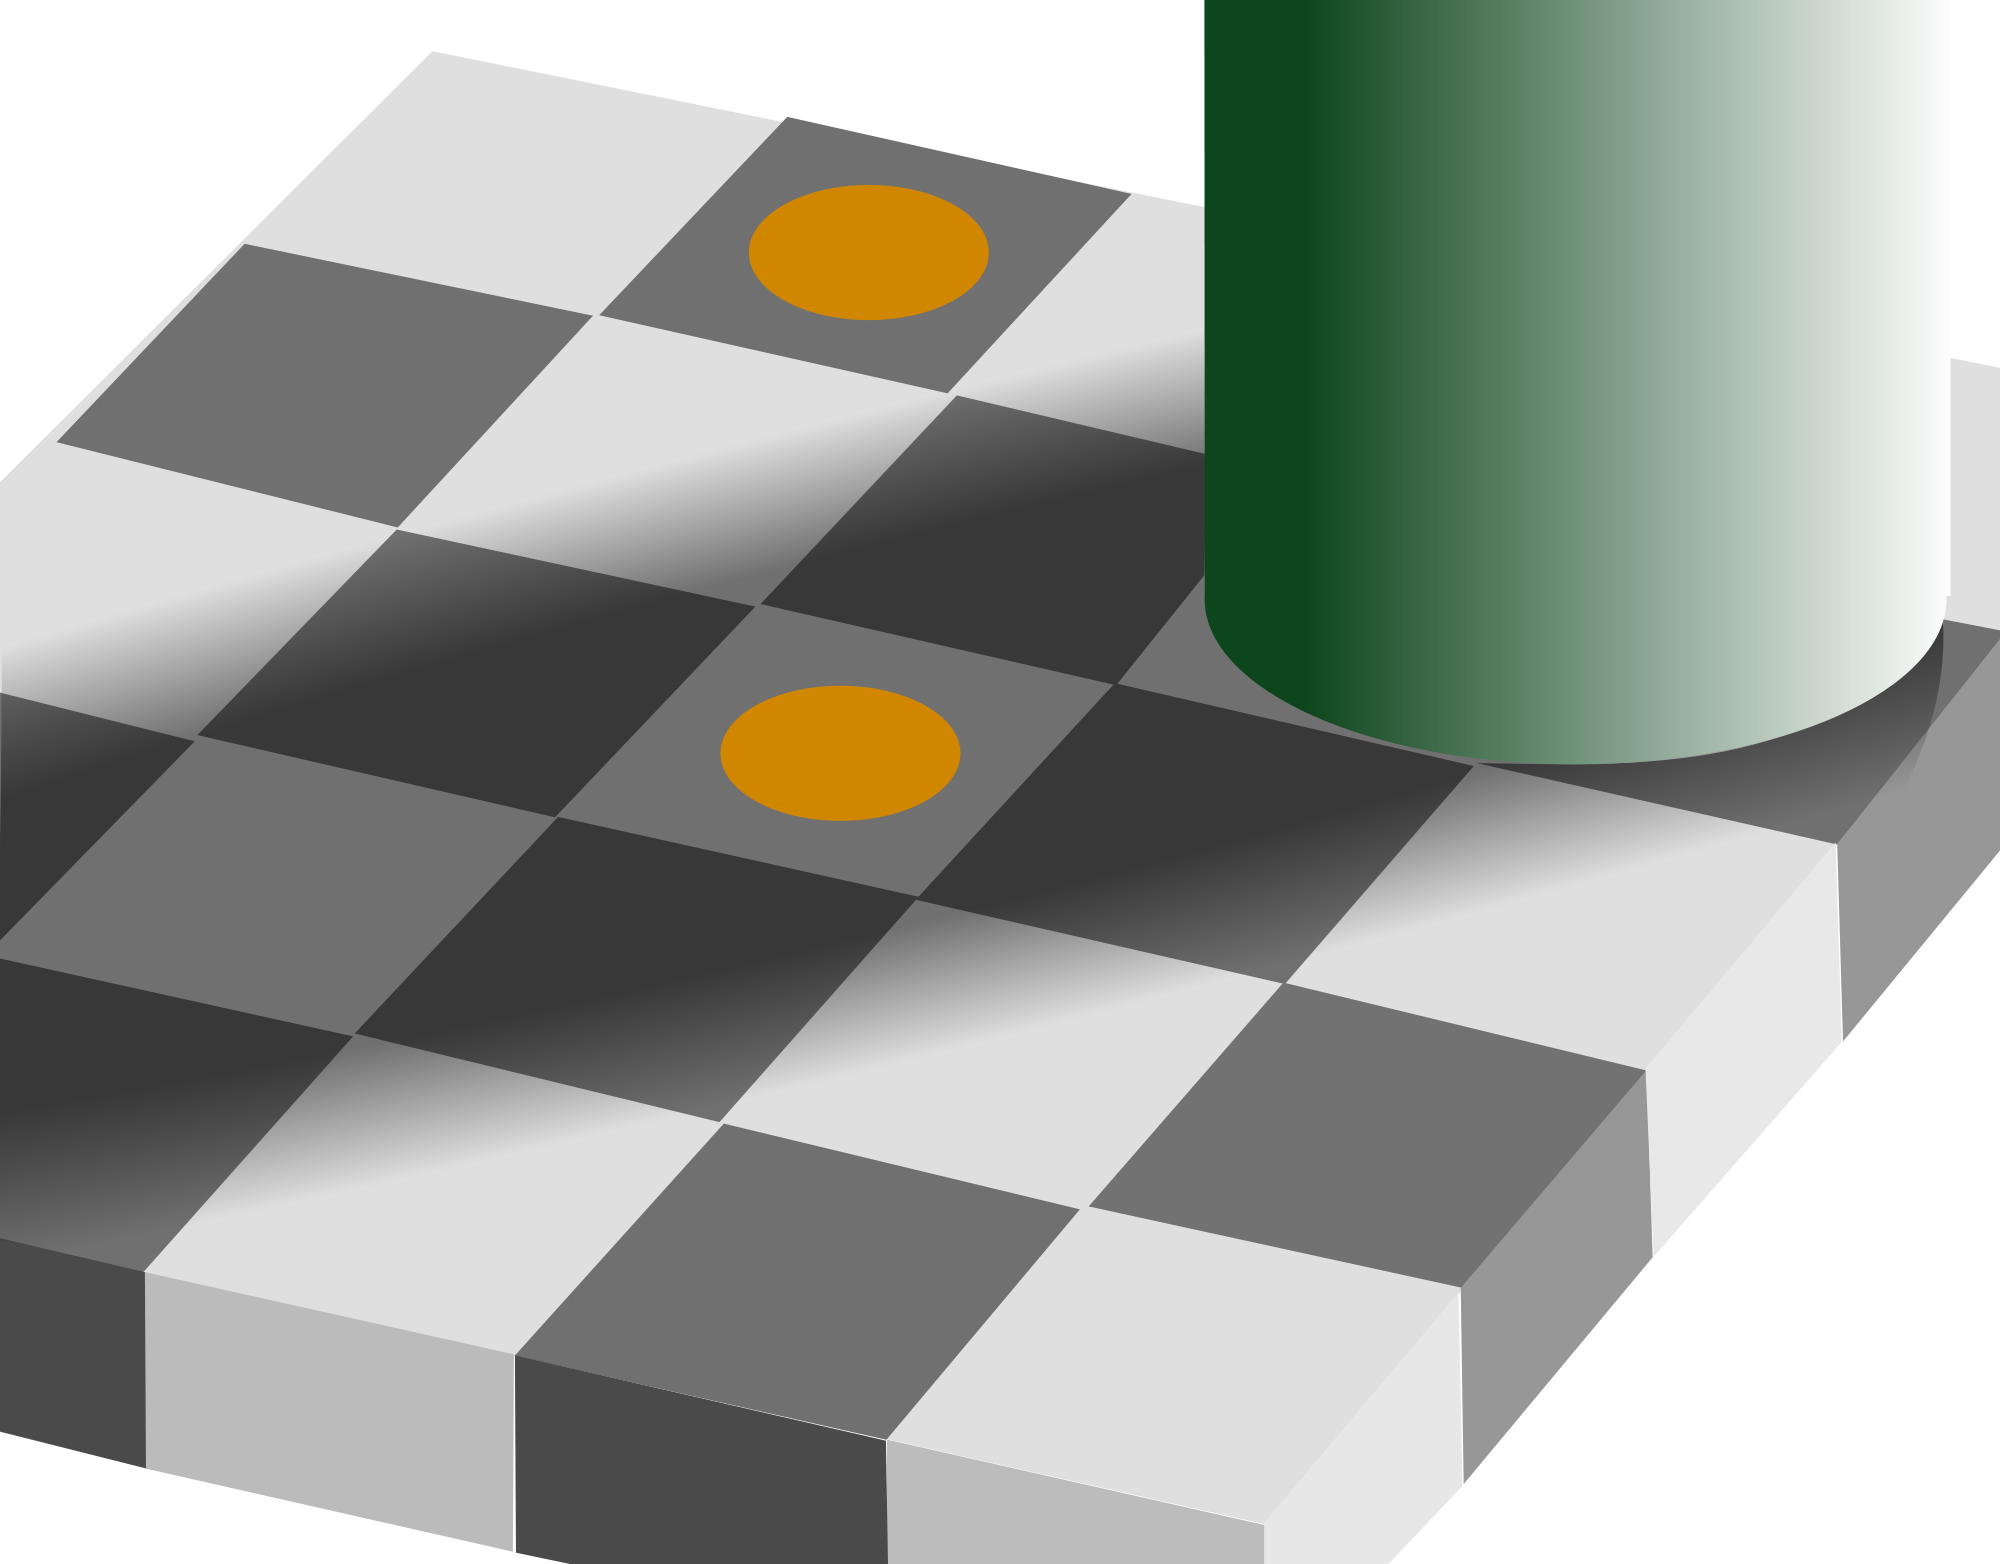
\includegraphics[width=50mm,height=50mm]{image01.png}
	\end{figure}
	
When it comes to faces there are two main ways illumination could degrade our images.  One, a uniform change in ambient 
light.  This occurs when the light source is straight on, visually the whole image gets darker or brighter.  Two, 
localised lighting changes, e.g. the light source is to the right of the face, so the left side is darker than the right.  
This is a distinction we will come back to later.  Illumination is clearly something any face recognition service will 
have to take into account if it wishes to accurately recognize a set of faces.  Thus, illumination is a logical and 
readily available normalization target to test the ease of use of my system.

\section{Comparing Two Methods}
The plan will be to test a newly proposed method of illumination correction, The Mean Illumination Estimation (MIE) 
~\cite{LuoaRINMBoMEfFR}, against something with proven results, namely, OpenCV's built-in histogram equalization.  We 
have the proposition put forward by ~\cite{LuoaRINMBoMEfFR} that their algorithm bests the current standard for 
illumination correction.  This implies that it should fare better than a simple quick and easy Histogram Equalization 
technique from OpenCV.

\subsection{Histogram Equalization}
As stated we will be employing OpenCV's implementation of this algorithm.  However, presented below is an overview on 
how the algorithm works and why it is theoretically useful to correct for different illumination conditions. \\

\pagebreak

Before we get into the math of the method an intuitive description would be useful.  Ideally what would happen using histogram 
equalization is given an image with 256 pixels and applying histogram equalization, one pixel will have a value of 1, another 
would have value 2, another would have value 255 etc.  Or if we had an image of 512 pixels, two would get a value of 0, another 
two would get 1 etc.  So a uniform distribution of pixel values is the goal.  However, doing so we would lose structure to our 
image as pixel values originally of the same intensity get mapped to different values ~\cite{urlIntuitiveHistEqualization}.  
So, at a minimum  we need to make sure that pixels of the same intensity value in the base image get transformed to the same 
``normalized'' intensity.  We also need to be careful that we don't affect the base structure of the image in another way i.e. 
pixel $(x_0, y_0)$ which is brighter than pixel $(x_1, y_1)$ put through this algorithm to get $(x'_0, y'_0)$ will still be 
brighter than $(x'_1, y'_1)$ though both values will likely have changed. \\

Mathematically we are mapping a clustered potentially non-uniform distribution to a wider (0-255) more uniform spread of 
intensity values.  Let $f$ be the given image represented by a $n \times m$ matrix of pixel intensities ranging from (0 to L-1) 
where $L$ is the number of possible values (usually 256) Now $p$ will denote the normalized histogram of our image $f$ as a list 
of bins per intensity value:

	\begin{equation}
		p_{n} = \frac{x_n}{Total} \quad n = 0,1,2,....,L-2, L-1
	\end{equation}
	
where $x_n$ is the number of pixels with intensity 'n' and 'Total' is the total number 
of pixels in the image.  We will define the Histogram equalized image as 'g';

	\begin{equation}
		g_{ij} = floor((L-1)\sum_{n=0}{f_{ij}} p_n )
	\end{equation}
	
Note floor rounds down the value.  The explanation used here can be found from the University of California 
~\cite{urlHistEqualization}

\subsection{Summary of Histogram Equalization}
Now we have a normalised image with which we can hopefully perform recognition on with greater success.  We note that technically 
it doesn't really care that there are illumination issues present.  Histogram equalization is a global image operation that will 
effect the entire image in the same way, regardless of the actual lighting conditions present in portions of the image.  i.e. if we 
took a face image with one half bright and one half dark and put it through the algorithm, as already stated above, the brighter 
pixels on the one half will still be brighter after the equalization is performed which still equates to an illumination problem 
for the Eigenface algorithm.  However, these are very much edge cases.  For the most part illumination issues will be of the form 
of global lighting differences.


\subsection{Mean Illumination Estimation}
	This method takes a localised smoothing approach to lighting normalization.  This is done so as to remove the components of 
	the image responsible for illumination changes.  Firstly it notes that according to the Illumination-Reflection model described 
	in detail in ~\cite{JianSaCSiIaSRCTaA}, a pixel $f_{xy}$ in a facial image gets its value from two components. $r_{xy}$ 
	represents the reflection component of an image at the point $(x,y)$ and $i_{xy}$ represents the illumination component.  Thus 
	we get the equation:
		
		\begin{equation}
			f_{xy} = r_{xy}	\times i_{xy}	
		\end{equation}
		
	Now, as $r_{xy}$ is dependant purely on the surface material in question and not affected by illumination it would be an 
	intrinsic representation of the facial image.  Suppose $i_{xy}$ changes little in value	within a small area while in the 
	presence of a weak light source.  The key idea now is to estimate the regional value of the illumination and use this to 
	cancel out the illumination. Thus we wish to find an estimate of our image $f_{xy}$ that will allow us to do this separation.  
	To attain such an estimate we apply a logarithmic transformation to each pixel in our image $f_{xy}$ we call this new function 
	$g_{xy}$
		
		\begin{align}
			g_{xy} &= ln(f_{xy}) \nonumber \\
			&= ln(r_{xy}) + ln(i_{xy})
		\end{align}
		
	Now $\hat{g}_{xy}$ becomes a mean estimate for $g_{xy}$ and is obtained via: 
		
		\begin{align}
			\hat{g}_{xy} &= \frac{1}{n^2} \sum_{(s,t)\in\omega_{nn}} g_{st} \nonumber \\
			&=  \frac{1}{n^2} \sum_{(s,t)\in\omega_{nn}} ln(r_{st}) + \frac{1}{n^2} \sum_{(s,t)\in\omega_{nn}} ln(i_{st})
		\end{align}

	Note $\omega_{nn}$ is the area around a given pixel $(x,y)$ with $(s,t)$ being the enumeration of these pixels and n is the 
	width/height of said kernel around $(x,y)$.  Next, the quotient image $d_{xy}$ is constructed from equations, (2.4),(2.5) we 
	do so to eliminate $i_{xy}$ (or make its contribution to the image negligible):
		
		\begin{align}
			d_{xy} &= g_{xy} - \hat{g}_{xy} 	\nonumber \\
			&= ln(r_{xy}) - \frac{1}{n^2} \sum_{(s,t)\in\omega_{nn}} ln(r_{xy}) + \sigma
		\end{align} 
		
	Where: $\sigma = ln(i_{xy}) -(\frac{1}{n^2})\sum_{(s,t)\in\omega_{nn}} ln(i_{st})$ we note that $\sigma$ will be a very small 
	value and can hence be omitted from (4) leaving us with the relation:
		
		\begin{align}
		d_{xy} &= g_{xy} - \hat{g}_{xy} \nonumber \\
		&\approx ln(\frac{r_{xy}}{(\prod_{(s,t)\in\omega_{nn}} r_{st})^{\frac{1}{\pi^2}} })
		\end{align}
		
	Now, $d_{xy}$ represents the ratio between the current point's reflectance and the average reflectance around it.  When the 
	materials in the localised kernel around (x,y) are the same $d_{xy}$ tends towards zero, but when they are different e.g. 
	facial skin and facial features $d_{xy}$ becomes notably none-zero.  Let us consider:
		
		\begin{equation}
			\alpha = \frac{1}{ab}\sum_{(x,y)\in f_{a \times b}} |d_{xy}| 
		\end{equation}
		
	With $a$ = number of rows and $b$ = number of columns in an image $f_{a \times b}$.  $\alpha$ will represent the average grey 
	value ratio of the whole image and features.  Each pixel is hence expressed as the ratio exponent relative to the average grey 
	value:
		
		\begin{equation}
			h_{xy} = \exp{\frac{d_{xy}}{\alpha \dot \beta}}
		\end{equation}
		
	With $\beta$ being a controllable scaling factor.  However, it is usually set in the range of two to three.  Finally to improve 
	contrast and correct the resulting brightness level, highlight facial features and reduce impact of background noise, post 
	processing is done as:
		
		\begin{equation}
			\hat{o}_{xy} = \left\{
				\begin{array}{l l}
					h_{xy} 	& \quad h_{xy} < 1 \\
					1 		& \quad h_{xy} \geq 1
				\end{array} \right.
		\end{equation}
		\begin{equation}
			o_{xy} = [\frac{255 \times (\hat{o}_{xy} -c)}{1-c}]
		\end{equation}
		
	With $o_{xy}$ being the final result image to be used in training or recognition.  $c$ is the minimum value of $\hat{o}_{xy}$.  
	The math may be complex but the idea is rather simple, given an image, we separate out the intensity factor from the structure 
	of the face, setting it to zero and rebuilding the face.  An example is provided below. 
	
		\begin{figure}[h!]
			\centering
			\caption{Mean Illumination Estimation images before and after applying MIE taken from~\cite{LuoaRINMBoMEfFR}\label{fig:MIE}}
			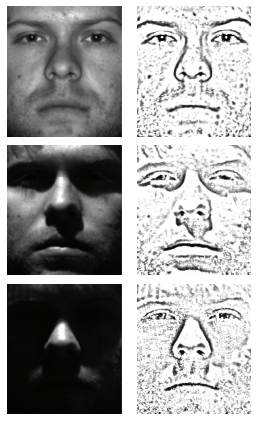
\includegraphics[width=75mm,height=120mm]{MIE.png}
		\end{figure}

	Notice here that the lighting angles have changed.  In the first image, the ambient light is full-frontal whereas the remaining 
	two images show shadows cast from various facial features ie directional lighting is present from this we gather the middle image 
	to be lit from about a 10'o'clock angle and the bottom image to be solely lit from above. \\
			
	The MIE algorithm leaves us with an image that for the most part is devoid of all extra light.  Ideally, multiple images of the same object 
	under different lighting conditions that are put through this algorithm will end up looking the same.  An example of it in use 
	can be seen below.  Note how, in the above fig:[~\ref{fig:MIE}], despite the drastic differences in illumination on the before 
	images, the right side varies little from face to face. \\
		
	The above images were 168x192 in size and it was discovered that for this size an n of 11 was optimal along with $\beta = 2.2$ 
	where $\beta$ is affected by facial reflectance of the subjects tested on.  However, it stays at a value of 2.2 as the facial 
	reflectance of different people varies little.
		
\subsection{Summary of Mean Illumination Estimation}
	The complications arise from estimating the illumination component so as to subtract it from the image, highlighting the remaining 
	reflectance of the image.  We achieve this by a logarithmic transform which only slightly (computationally) affects 
	the image, the fact remains that it still does change the image. \\
		
	In conclusion, any attempt to normalize an image's illumination will undoubtedly degrade some aspects of the image we would rather 
	retain.  However, one would hope that the gained standardization of facial images out way this degradation and yield more accurate 
	recognition rates.  We also note that this method is a localised correctional algorithm.  That is to say the afore mentioned issue 
	with histogram equalization not being very effective for images with half bright, half dark faces doesn't apply here.  The formula 
	and reasoning were put forward by and learned from ~\cite{LuoaRINMBoMEfFR}, an article that attempts to find a better way of solving 
	the lighting issue with positive results for their effort. \\
	
	Using the workstation, the task now is to gain more insight into the algorithm by attempting to duplicate the literature results 
	and to further validate the strengths and weaknesses of the algorithm.  The completed implementation of this algorithm in Python 
	can be seen in appendices:[A.1,A.2].  Note that little effort was made to optimise the program as the 
	implementation of the algorithm was a trial run to determine if the method would be useful for the system and our needs.  If the 
	algorithm does prove to be valuable, there are a number of means to improve efficiency as discussed at the end of the chapter.

\subsection{Validation of MIE implementation}
	Before the experiment can be run we first attempt to validate that aspects of the system work as intended.  
	This is done to provide validation to the results obtained from the experimental procedure.  Though we 
	predominantly wish to do so for our implementation of the Mean Illumination Estimation, for completion, we  
	also confirm OpenCV's built in Histogram Equalization method works as intended.

		\begin{figure}[H]
			\centering
			\caption{My MIE implementation [col 3] tested against provided example from ~\cite{LuoaRINMBoMEfFR} [col 2] \label{fig:MIE_Compariosn}}
			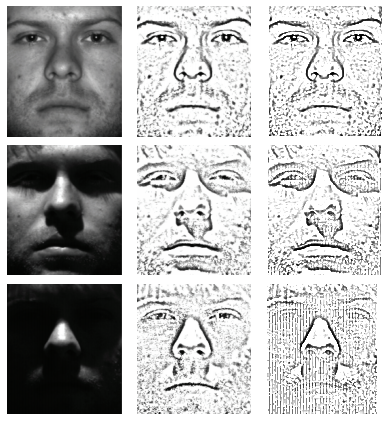
\includegraphics[width=75mm,height=80mm]{MIE_Compariosn.png}
		\end{figure}

	To start, we compare the output my MIE implementation provides against that of the output attained according 
	to ~\cite{LuoaRINMBoMEfFR}.  We note above in fig:[~\ref{fig:MIE_Compariosn}]; \\
	 
	We observe that my implementation provides near identical results to that of the article for the base face.  However, 
	as the images become darker our results seem to deviate more from those in the published paper.  We postulate that 
	these artefacts are being generated from the conversion between image to PDF used in the published paper, and back 
	to image again i.e. slight smudging and some significant frequency artefacts are introduced in the dark regions 
	from the conversion algorithm, possibly from compression algorithms. \\

	To confirm our hypothesis, here are several more images put through my algorithm that are not extracted from the PDF
	paper of ~\cite{LuoaRINMBoMEfFR}.  We see none of the below show similar artefacts to those found in 
	fig:[~\ref{fig:MIE_Compariosn}].

		\begin{figure}[H]
			\centering
			\caption{MIE implementation applied to CSC Honours 2015 Class list, Rhodes University. Some blacked out due to lack of permission from subjects\label{fig:MIE_training_data_from_my_method}}
			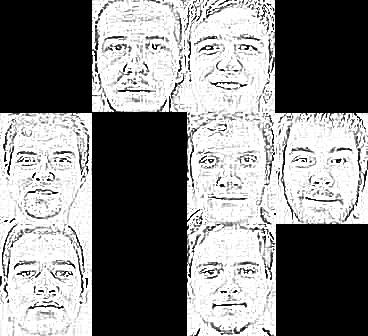
\includegraphics[width=120mm,height=115mm]{MIE_training_data_from_my_method.png}
		\end{figure}
	
	To further investigate, we took the original PDF images from the paper~\cite{LuoaRINMBoMEfFR} and ran them through the OpenCV implementation 
	of histogram equalization Below fig:[~\ref{fig:Hist_example}], we see the same faces as the MIE comparison test 
	fig:[~\ref{fig:MIE_Compariosn}] above.  However, instead of the MIE applied to them they have undergone histogram 
	equalization, an OpenCV algorithm in which there is a high confidence.

		\begin{figure}[H]
			\centering
			\caption{Histogram Equalization applied to article example faces~\cite{LuoaRINMBoMEfFR} \label{fig:Hist_example}}
			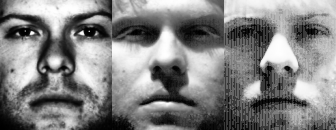
\includegraphics[width=100mm,height=40mm]{Hist_example.png}
		\end{figure}
		
	We see that the intensities have been stretched for all images, improving visibility, We also note in the middle 
	image around the eyes and in the far right image, once again the same artefact pattern emerges.  This points again 
	to an issue with the image itself, not the algorithms performed upon them.  \\
	
	Now that we have built confidence in our implemented code that it does work as intended by the original creators 
	we can construct an experiment to test the effects on accuracy they have.
	
\section{Reading The Graphs}
The algorithm ``classifies'' a face provided the matcher gets a ``deviation'' score less than the provided threshold.   Therefore 
at each threshold point we get three regions; going up; the first region defines the number of successfully classified images, 
the second region shows the number of unsuccessful classifications and the remaining portion of the graph are those images that 
were not yet classified under the current threshold but may still be under the next threshold level. 

\newpage
\section{A word on training}
We train the eigenface method with multiple images per subject.  This is done to increase accuracy of the system.  Having 
multiple images of the same person under different conditions provides a higher likelihood for the system to correctly match 
a new face to one of the subjects training data.  E.g. we train with 10 subjects, each subject has 5 training images one 
looking up, down, left, right and full-frontal we label each image as subject 1.  Thus, given a new image of the subject 
looking left, there is a higher probability for a successful match to subject 1 as the system has a training image of that 
subject looking left.

\section{Experiment 01: Setup}
First up we will test our system against the AT\&T database, this database contains 40 subjects with 10 images per subject 
totalling 400 images~\cite{ATTDATA}.  We have evenly split this data into training and test data i.e. 5 images per subject goes to 
training and the other five to test data.   The results we will be comparing are the total number of correct connections 
made by the Eigenface algorithm.  This database primarily focuses on orientation of the subjects faces and has limited 
illumination variance, as such, we expect the Eigenface algorithm to perform with some degree of accuracy and the application 
of our two normalisation techniques to have minimal if any effect on the accuracies obtained. 

\subsection{Experiment 01: Results}
We start with a base line, no normalization techniques used, just the plain dataset run through the 
Eigenface algorithm.  Doing so we get the graph;

	\begin{figure}[H]
		\centering
		\caption{Base line, no illumination normalization used; AT\&T \label{fig:Att_BaseLine}}
		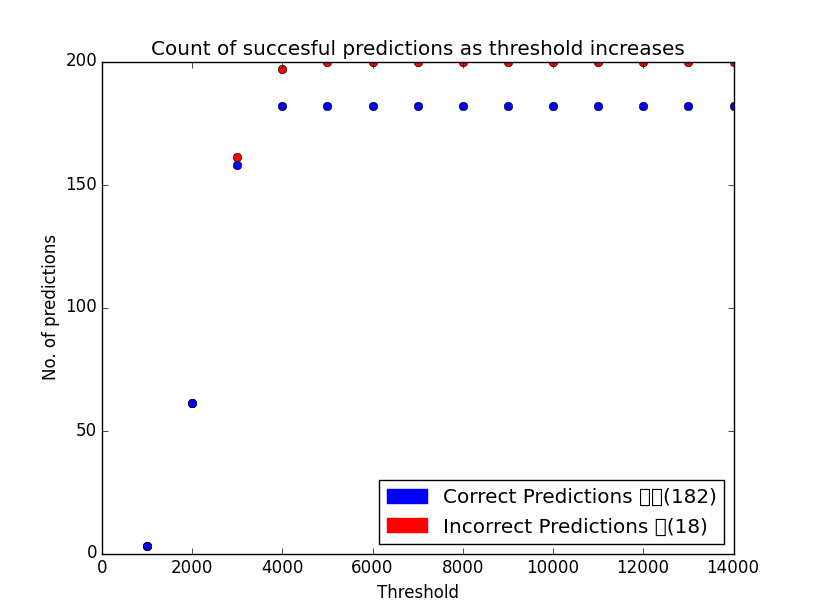
\includegraphics[width=100mm,height=70mm]{Att_full_None.png}
	\end{figure}

From Figure:~\ref{fig:Att_BaseLine} we see that we correctly recognize $\frac{182}{200}$ subject images i.e. equating to a 
91\% accuracy.  We run the experiment again but this time perform histogram equalization upon both test and training data.  
This provides us with the graph; 

	\begin{figure}[H]
		\centering
		\caption{Histogram Equalization experiment; AT\&T \label{fig:Att_Hist_exp}}
		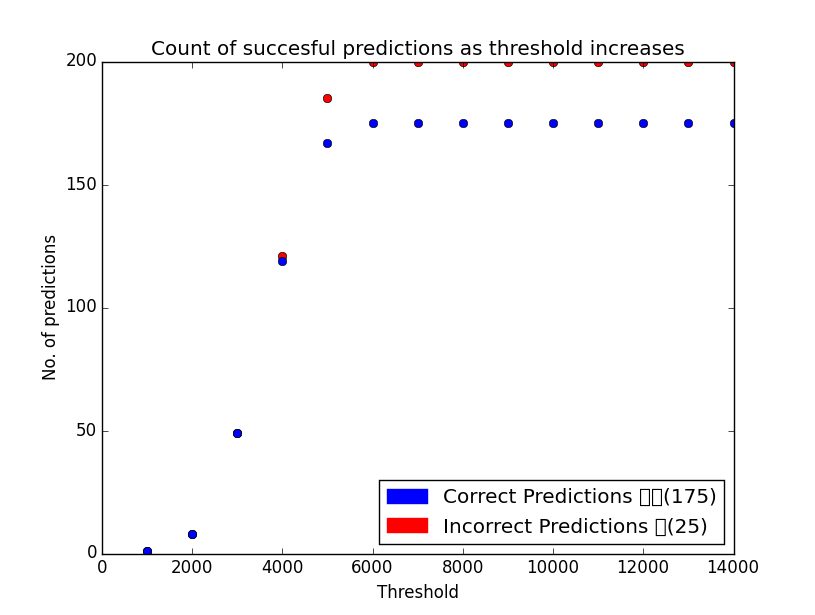
\includegraphics[width=100mm,height=70mm]{Att_full_Hist.png}
	\end{figure}
	
We now see from Figure:~\ref{fig:Att_Hist_exp} that the system can correctly recognize $\frac{175}{200}$ of the subject images,
roughly 87\% accuracy rating, a slight drop from the base line but still a viable accuracy.  we also note that it is significant 
that at lower threshold values, almost no incorrect classifications are made.  As we increase the threshold after about 80\% 
correctly classified, the final 20\% have about an equal number of correct and incorrect classifications occur.  
We now run the experiment again.  However, now we test our MIE algorithm.  Doing so, we obtain the results;

	\begin{figure}[H]
		\centering
		\caption{MIE experiment; AT\&T \label{fig:Att_MIE_exp}}
		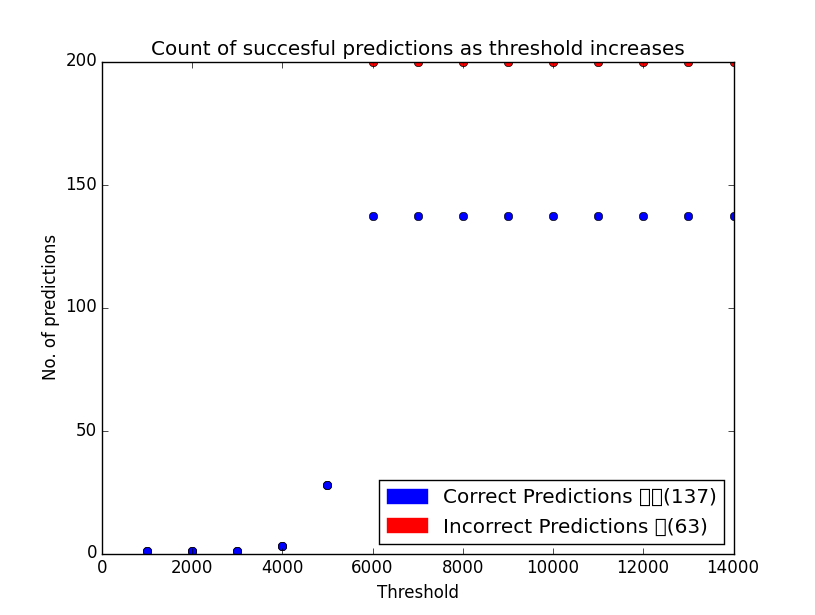
\includegraphics[width=100mm,height=70mm]{Att_full_MIE.png}
	\end{figure}

Here we see greatly diminished results with, $\frac{137}{200}$ recognized faces, equating to roughly 68\% accuracy.  Once again, 
we try two more experiments, 1.) we run histogram equalization first, then MIE upon this normalised data. 2.) the other way round, 
test MIE first, then histogram equalization;
 
 	\begin{figure}[H]
		\centering
		\caption{Histogram then MIE; AT\&T \label{fig:Att_Hist_MIE_exp}}
		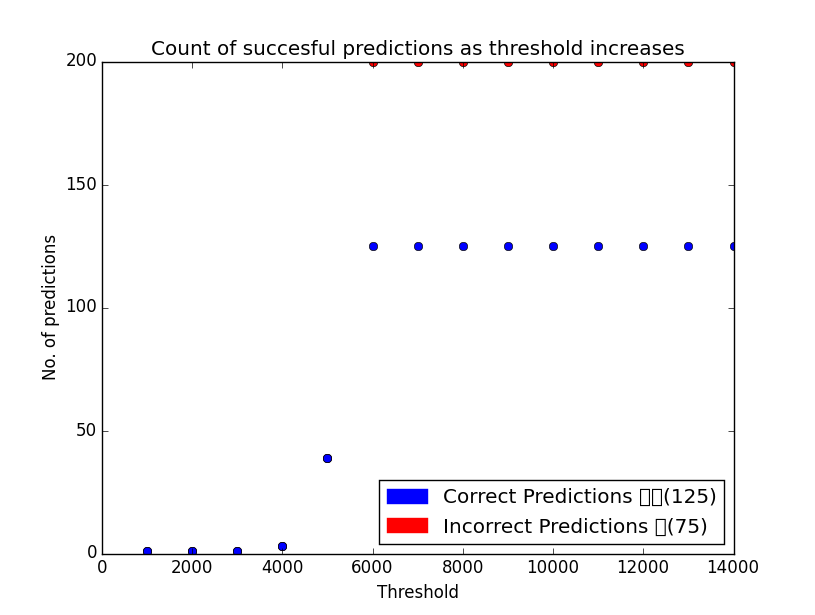
\includegraphics[width=100mm,height=70mm]{Att_full_Hist_MIE.png}
	\end{figure}
	
   	\begin{figure}[H]
		\centering
		\caption{MIE then Histogram; AT\&T \label{fig:Att_MIE_Hist_exp}}
		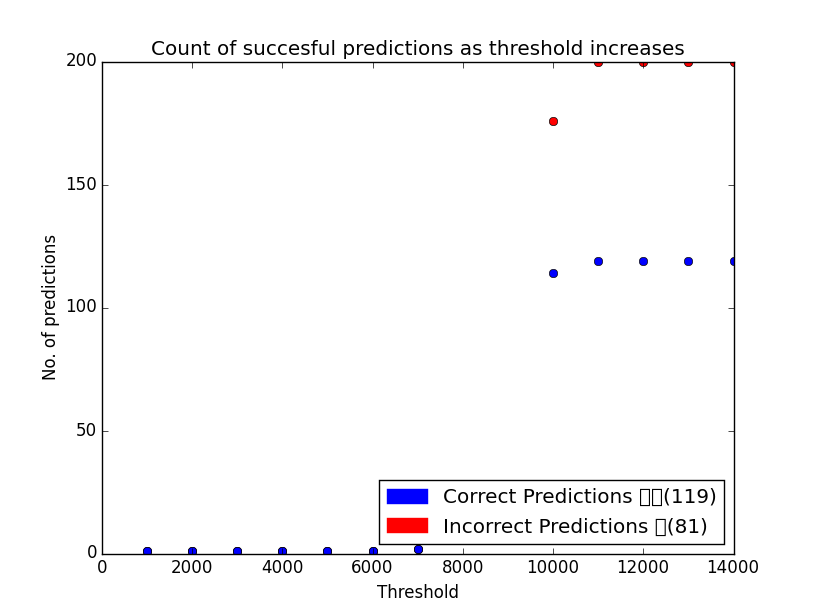
\includegraphics[width=100mm,height=70mm]{Att_full_MIE_Hist.png}
	\end{figure}
  
Aside from the over all inaccuracy of the combination we see a connection emerge; histogram equalization then MIE performs 
in accordance with MIE on its own if slightly less accurate but the other way round provides far worse results.

\subsection{Experiment 01: Discussion}
Initially we observed what we expected, the baseline performed with a high degree of accuracy due to the lack of illumination 
change in the images.  However, to our disappointment when we run our correction algorithms we see diminished results with 
MIE being completely impractical for normal use.  \\

\section{Experiment 02: Setup}
For this experiment the conditions were; Yale B face database ~\cite{KCLee05} which contains 38 individuals with 65 images per 
subject (2470 total).  However, to reduce computation time I will only used a subset of the data, the first 20 subjects. Note, 
the Eigenface algorithm cannot handle images of varying size,  so many of the subjects have images that need to be discarded as 
they are larger than the others panned out larger and needing to be cropped.  Also, some of the images were provided as corrupt, 
presumably as further testing data, they too have been removed.  Furthermore we also take 10 images per subject to use as the 
training set.  What remains is 20 subjects and 1072 images as testing data.  The results we will be comparing are the total number 
of correct connections made by the Eigenface algorithm.  Based on the literature and as noted above, we expect MIE to surpass 
OpenCV's Histogram equalizations recognition accuracy.

\subsection{Experiment 02: Results}
As before we start with a base line, no normalization techniques used, just the plain dataset run through the 
Eigenface algorithm.  Doing so we get the graph:

	\begin{figure}[H]
		\centering
		\caption{Base line, no illumination normalization used; Yale B\label{fig:BaseLine}}
		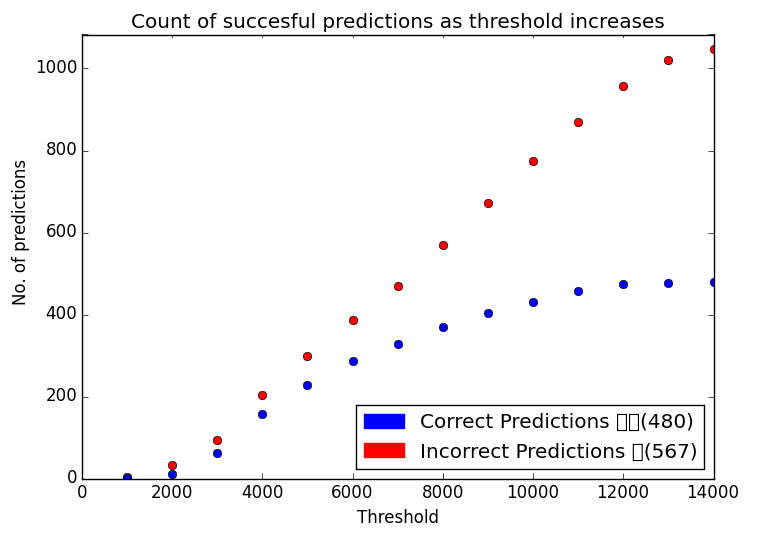
\includegraphics[width=100mm,height=70mm]{Yale_half_None.png}
	\end{figure}
By contrast to the previous dataset, here we see incorrect classifications even at low threshold values and a flat-lining of 
the correct predictions graph i.e. increasing the threshold will give more inaccurate classifications then correct ones.
From fig:[~\ref{fig:BaseLine}] we see that we correctly recognize $\frac{480}{1072}$ subject images i.e. roughly 45\% 
accuracy.  We run the experiment again but this time perform histogram equalization upon both test and training data.  
This provides us with the graph; 

	\begin{figure}[H]
		\centering
		\caption{Histogram equalization experiment; Yale B \label{fig:Hist_exp}}
		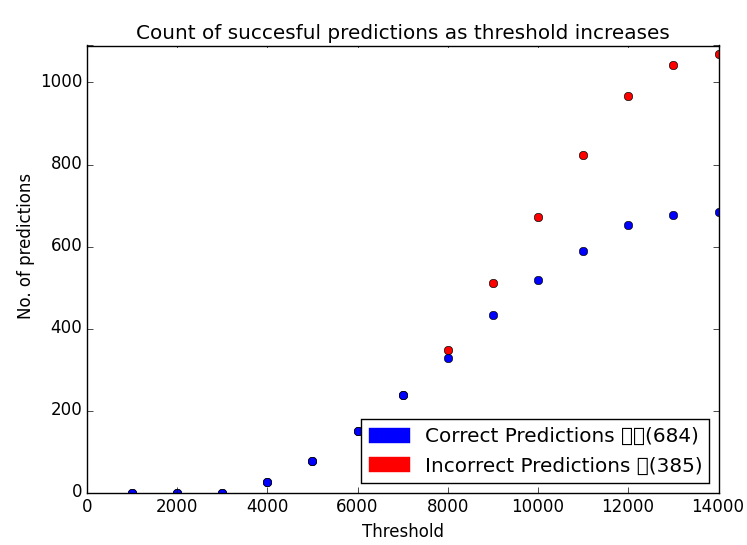
\includegraphics[width=100mm,height=70mm]{Yale_half_Hist.png}
	\end{figure}
	
We now see from fig:~\ref{fig:Hist_exp} that the system can correctly recognize $\frac{684}{1072}$ of the subject images, 
roughly 64\% accuracy rating, a meaningful improvement on the base line.  \\

We now run the experiment again.  However, instead of Histogram Equalization, we test our MIE algorithm.  Doing so, we obtain 
the results.

	\begin{figure}[H]
		\centering
		\caption{MIE experiment; Yale B \label{fig:MIE_exp}}
		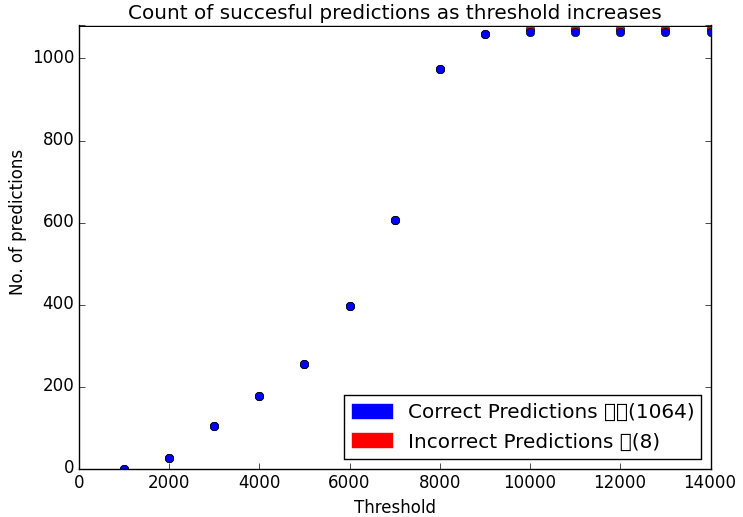
\includegraphics[width=100mm,height=70mm]{Yale_half_MIE.png}
	\end{figure}

Here we see greatly improved results with, $\frac{1064}{1072}$ recognized faces, 
equating to roughly 99\% accuracy. \\ 

In a final attempt to yield even better results, we performed two more experiments, 1.) we run histogram equalization first, 
then MIE upon this normalised data. 2.) the other way round, apply MIE first, then apply histogram equalization.
 
 	\begin{figure}[H]
		\centering
		\caption{Histogram then MIE; Yale B \label{fig:Hist_MIE_exp}}
		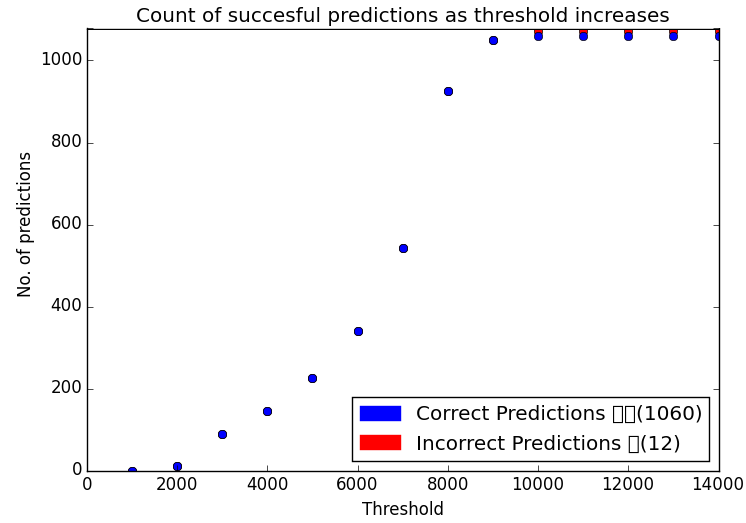
\includegraphics[width=100mm,height=70mm]{Yale_half_Hist_MIE.png}
	\end{figure}
	
   	\begin{figure}[H]
		\centering
		\caption{MIE then Histogram; Yale B \label{fig:MIE_Hist_exp}}
		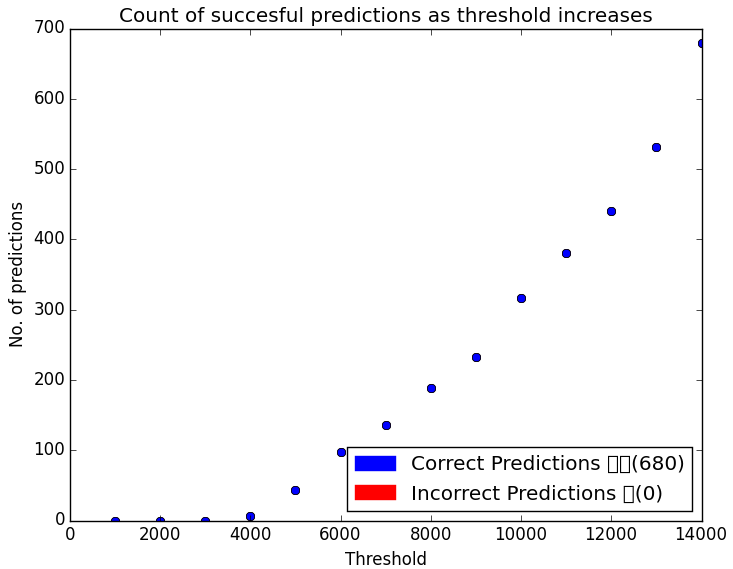
\includegraphics[width=100mm,height=70mm]{Yale_half_MIE_Hist.png}
	\end{figure}
  
We see from these experiments that Performing Histogram Equalization first and then MIE on top of that performs nearly as 
well as MIE on its own, but the other way round yields shocking results, failing to even score all images under the maximum 
14000 threshold.  It is significant though, that this combination makes very few misclassification (None, in fact, in fig:~\ref{fig:MIE_Hist_exp})

\subsection{Experiment 02: Discussion}
The Baseline experiment, fig:[~\ref{fig:BaseLine}] provides a very poor score with this facial database, this was to be 
expected due to the high impact of lighting conditions on the Eigenface algorithm, yielding a score of $\frac{480}{1072}$, 
roughly 45\% accuracy.  On top of that, it technically doesn't even score all the images, 3 were missed i.e. their threshold 
values were higher than the upper limit of our graph. \\

The first experiment we try is histogram equalization.  Here we see an improvement in recognition at roughly 64\%.  We 
already know from the explanation of the workings of histogram equalization that it is not ideal for the Eigenface
method when used on images with localised lighting conditions, something that the Yale B database has in abundance.  
This aside, all in all, it is a notable improvement on the none-normalised score but still far from the ideal. \\

Next we hope to achieve better results with the MIE version of the data.  We get results which far surpass those provided 
by histogram equalization, at roughly 99\%. This is because the MIE is a very localised oriented algorithm and as the Yale B 
database has nearly insignificant change in orientation and angle, purely lighting changes, the MIE performs well.  
As such, these results most certainly agree with the claim published in~\cite{LuoaRINMBoMEfFR}. \\

With regards to the compound tests I deduce the reason for such discrepancy between the order is that performing histogram 
equalization first outputs a very lightly affected image with just a simple contrast change that MIE can operate on in much 
the same way as before, while trying to do it the other way, MIE outputs a vastly different image from the original, more 
resembling a sketch than a photo, with large variation in colour intensities,  as such the histogram equalization algorithm 
falters as we have reduced the colour space to an even more compact region of the spectrum.  Thus when we pass these new 
images through the histogram equalization method it just does more damage by stretching it further.  \\

What we take away from this is that although MIE performs phenomenally against strong illumination conditions it tends to 
degrade the image it is working on to an extent that other normalization techniques are ineffective at best and further 
degrading at worst. \\

In reality we probably wouldn't want to perform multiple normalization techniques that target the same issue upon our dataset 
as we would expect such conflicts to arise.  On the other hand we would hope that combining these techniques with others that 
target different aspects of normalization would not conflict with each other.  Indeed, we would hope that doing so would provide
a higher degree of accuracy in recognition.


\section{Summary}
This chapter confirms the claim made earlier that the Eigenface algorithm is very sensitive to lighting fig:[~\ref{fig:BaseLine}]
showed very low recognition rates, yet the same data improved spectacularly after MIE was applied fig:[~\ref{fig:MIE_exp}] \\

To conclude, yes, MIE looks good, but only for a narrow category of normalization problems namely, those with localized regions of 
lighting variation on that note, I find it hard to believe any algorithm could improve upon those accuracies.  Sadly that's where the 
downsides must be mentioned.  The algorithm doesn't play well with other techniques and even less so when there are no local 
illumination issues present, tending to be more of a hindrance than a help.  Taking note of this, for our implementation in classroom 
attendance tracking, we have a semi-controlled environment where lighting conditions will be more along the lines of uniform 
differences across our subject faces.  As such OpenCV's histogram equalization would be the algorithm of choice for our needs.  \\

The very low rate of miscalculations using the combined algorithms might have uses elsewhere.  In some scenarios a ``false classification'' 
might be very costly - i.e. In airport security, it would require pulling the individual from the queue for further interrogation. \\

The Python implementation of MIE was horribly time inefficient.  As a benchmark, OpenCV's histogram equalisation was performed 
upon the 1272 images and did so in under a minute while my Python implementation of MIE took roughly 10hrs to do the same number of images. 
Again, this speed difference comes with the benefit of being a very localised method.  Each pixel is compared to a 11x11 kernel 
around itself as well as the average intensity for the whole image.  This means it can handle images which are dark on one side but 
light on the other without problems. \\  

It was beyond the scope of this work to attempt to optimise this method. However, we do note the following possible optimisations; \\
1.) Converting the MIE code logic into C++ or C that is then wrapped into Python, doing so could offer substantial speed-ups. \\
2.) The current implementation is fairly naive: the 11x11 region is recomputed for each pixel in the image.  Many efficient image 
processing algorithms operate by sliding a difference window over the image and computing a running estimate of local intensity in 
our case we would reduce the 121 computations to 22 per pixel.  This would most certainly improve the performance of the method. 
Finally, this per pixel kernel methodology indicates that this method could see a large speed-up if performed through a GPU.  
However, these are ideas for future work to look into.




	
	% chapter detailing all nmerical results 
	% obtained through various experiments done 
	% both along the way and upon compleation 
	% of my system.
	\chapter{Assignment Problem}
	\section{The Problem}
Now that we have determined a sensible illumination normalization technique to use, we turn our 
attention to another means of improving recognition rates.  When we consider the problem we are
trying to solve, namely facial recognition for classroom attendance tracking, we realise that 
the current method of classification used by the Eigenface method doesn't make any use of the 
intrinsic properties of our problem. \\

We know exactly who and how many subjects should present in each lecture.  Knowing this, we can 
in theory improve our recognition rates by doing away with Eigenfaces current greedy, first match 
algorithm and in its place use a global assignment algorithm like the Hungarian Algorithm which 
we shall look into in the following sections. \\

The following chapter discusses but does not implement the following features due to constraints 
that are discussed at the end of the chapter.  In its current state the provided Eigenface 
algorithm makes use of a greedy first match algorithm.  When you don't know the sets you are dealing 
with and whether or not the face you are testing is even in your data set, it is a adequate solution.  
It will take a test face and try find the best match it can in its training data as well as providing 
a matching confidence.  \\
	
However, we do know the sets, and are sufficiently confident that every face we test is in our training 
data.  Thus we can surely use this knowledge by making use of a multiple assignment optimisation 
algorithm.  Such an algorithm scores every test face against all training faces, thereafter, optimise 
the classification of who's who to minimize the total score of the entire classification.

\section{The Assignment problem}
The assignment problem details the complexity of assigning two sets to one another such that some cost 
is minimised.  Doing so has many real world applications; Logistics of Assigning cargo to ships/trucks 
to minimise fuel costs based on their varying shipping/land routes~\cite{Assignmentproblems}, assigning 
jobs to various employees to yield the least possible wage expense etc. 

  	\begin{figure}[H]
		\centering
		\caption{The Assignment problem \label{fig:Assign_part1}}
		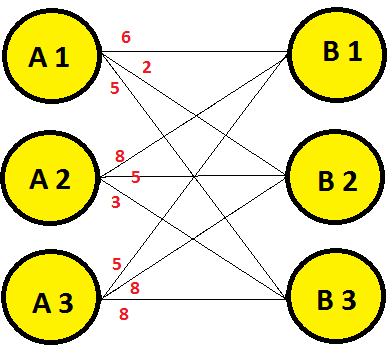
\includegraphics[width=95mm,height=95mm]{Assign_part1.png}
	\end{figure}
	
Above in fig:[~\ref{fig:Assign_part1}] details a problem of assigning set A to B we see that each 
connection has an associated cost involved.  We note each branch varies in cost thus mathematically, 
different selections would have different costs incurred, hence there must exist one selection that 
has a cost less than or equal to all other combinations. 

  	\begin{figure}[H]
		\centering
		\caption{The Assignment problem solution \label{fig:Assign_part2}}
		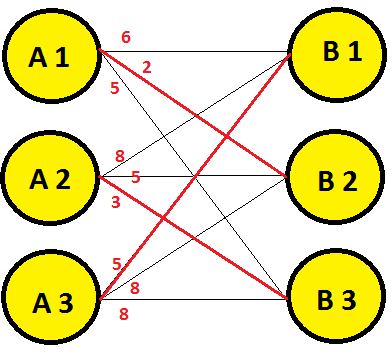
\includegraphics[width=95mm,height=95mm]{Assign_part2.png}
	\end{figure}

We see from fig:[~\ref{fig:Assign_part2}] that the cheapest matching is the selection [A1,B2],[A2,B3],
[A3,B1] now doing this by eye was trivial enough for these sets.  Now what if we had 100 elements per 
set?  Clearly what we need to do is find an algorithm that can solve this problem for us within a 
reasonable time.  To this end, we look at the Hungarian Algorithm~\cite{Hungarian_alg}.
 
\section{Hungarian Algorithm}
The Hungarian Algorithm is a proposed solution to the assignment problem that is solved by minimizing the 
total costs of all assignments.  Since Eigenface matching measures the difference between the feature 
vector of a probe face compared to the feature vectors of the training faces, a close match returns a low 
number.  So for our problem, we wish to minimise the overall difference.  As we work with a matching score that 
is better the smaller it is, we have a classic minimisation problem to which the Hungarian Algorithm is well 
suited. \\

In order for the algorithm to work it needs to be able to build up a square matrix i.e. the two sets you 
wish to match must be of the same length.  With this in place we would score the data, putting the 
confidences attained in an output matrix $m_{n \times n}$.  The element $m_{i \times j}$ where $i,j < n$ 
of the this matrix would then indicate the Eigenface score of probe feature vector $i$ against the feature 
vector of the training face $j$.  Now the problem involves choosing a combination of scores such that the 
total combination of these scores is as small as possible. \\

One point we need to take into account is the situation where we have less students present than there 
should be or the less likely situation where there are more.  These are concerns because as previously stated, 
the Hungarian Algorithm needs a square matrix to operate on.  We have two options: we can pad with high numbers 
or zeros.  Standard procedure is to pad the rows or columns with values equal to the highest present value 
currently in the matrix.  Thus those present get the best chance at matching the faces in the set i.e. the 
assignment of subject $n$ to training subject three with a confidence of 300 isn't stolen by one of our made up 
padded students who we gave a stronger match by setting the padding to 0. \\

We could do this by hand for small sets, but the problem quickly escalates as the sets become bigger 
in fact the problem done this way is of O(n!) not ideal.  However at the core of the Hungarian Algorithm 
is the theorem: If a number is added to or subtracted from all of the entries of any one row or column 
of a cost matrix, then an optimal assignment for the resulting cost matrix is also an optimal assignment 
for the original cost matrix ~\cite{Hungarian_alg}. This observation allows us to force the least cost 
in a row or column to be represented as a zero.  In turn, this provides an efficient way of ``eliminating'' 
rows and columns from the matrix to reduce the size of the remaining problem. \\

The algorithm from ~\cite{Hungarian_alg};
\begin{enumerate}
	\item Firstly, subtract the smallest entry in each row from all the other entries in that row.  Now do the same for each column. 
	\item Select rows and columns so that all zero elements are selected with the minimum number of selections. 
	\item (I) If the number of selections is n, then we are done, we have found the optimal assignment. \\
		  (II) If we have less than n selections an optimal selection is not yet possible, so we proceed. 
	\item Determine smallest entry not yet covered by any line, subtract this value from each element in every unselected row 
		  and add it to each element in each selected column.   Return to step 2.
\end{enumerate}

Below is a working example of the Hungarian Algorithm, given fig:[~\ref{fig:select_step_1}]
  	
	\begin{figure}[H]
		\centering
		\caption{Initial matrix \label{fig:select_step_1}}
		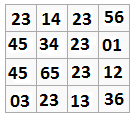
\includegraphics[width=50mm,height=50mm]{select_step_1_Hungarian.png}
	\end{figure}
	
Performing the first step (least value row subtraction) we get fig:[~\ref{fig:select_step_1_1}]

	\begin{figure}[H]
		\centering
		\caption{Subtraction of least value per row \label{fig:select_step_1_1}}
		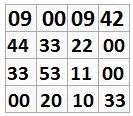
\includegraphics[width=50mm,height=50mm]{select_step_1_1_Hungarian.png}
	\end{figure}

Performing the second step (least value column subtraction) we then get fig:[~\ref{fig:select_step_2}]

  	\begin{figure}[H]
		\centering
		\caption{Subtraction of least value per column \label{fig:select_step_2}}
		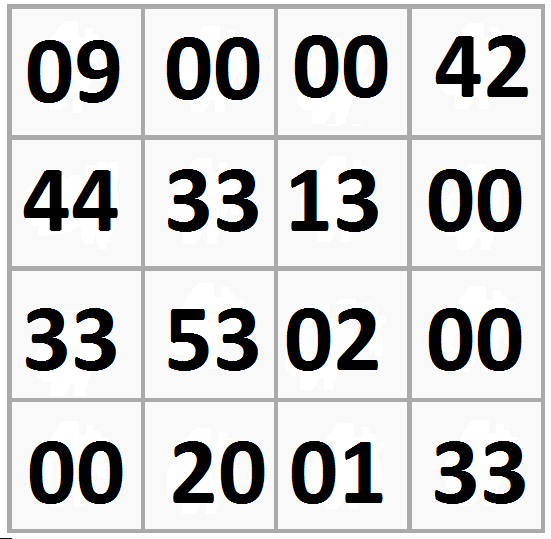
\includegraphics[width=50mm,height=50mm]{select_step_2_Hungarian.png}
	\end{figure}
	

So, mathematically, we can manipulate along rows or down columns by the same operation without it affecting
the integrity of the matrix.  We know this thanks to the afore mentioned theorem the proof of which is 
beyond the scope of this work.  However, we have another aspect to look at, how exactly do we find the 
minimum selection of rows/columns that contain all our zeroed elements? One way this can be done is as 
follows; \\

\begin{itemize}	
 \item First as seen in fig:[~\ref{fig:select_step_3}], make as many minimum cost assignments as possible 
 without double assigning.  In the provided example we have designated this with an apostrophe.  We select 
 [4,1] as an option as it has no conflicts.  However, for row 1 we need to make a choice, this choice can 
 safely be made arbitrarily.  Doing so we select [1,2] instead of [1,3] similarly we must choose between 
 [2,4] and [3,4] we choose [2,4].
\end{itemize}

  	\begin{figure}[H]
		\centering
		\caption{Selection of rows and columns step 1 \label{fig:select_step_3}}
		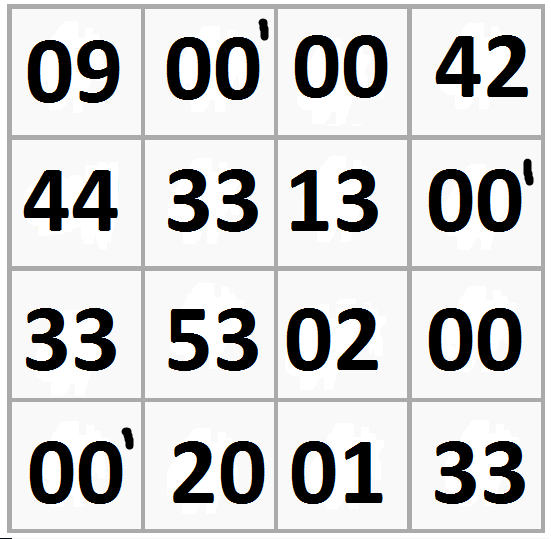
\includegraphics[width=50mm,height=50mm]{select_step_3_Hungarian.png}
	\end{figure}

\newpage	
Step 2:
\begin{itemize}
 \item Now, mark all rows having no assignments (zeros marked with apostrophes) (row 3) Shown as (X1) in the following diagram
 \item Next, mark all unmarked columns having zeros in newly marked rows (column 4) (X2)
 \item mark all rows having assignments in newly marked columns (row 2) (X3)
\end{itemize}

Doing the above we end up with fig:[~\ref{fig:select_step_4}] 

  	\begin{figure}[H]
		\centering
		\caption{Selection of rows and columns step 2 \label{fig:select_step_4}}
		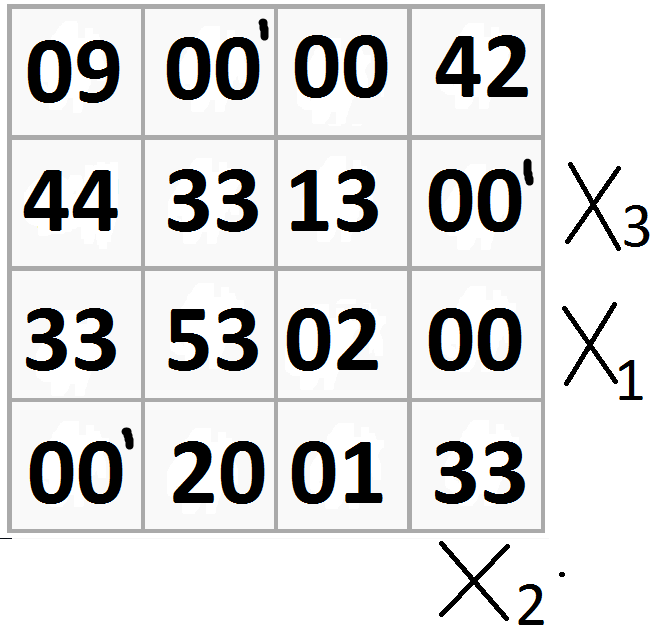
\includegraphics[width=50mm,height=50mm]{select_step_4_Hungarian.png}
	\end{figure}

\begin{itemize}	
 \item Finally make your selections on all marked columns and all UNMARKED rows.  
\end{itemize}

  	\begin{figure}[H]
		\centering
		\caption{Selection of rows and columns step 3 \label{fig:select_step_5}}
		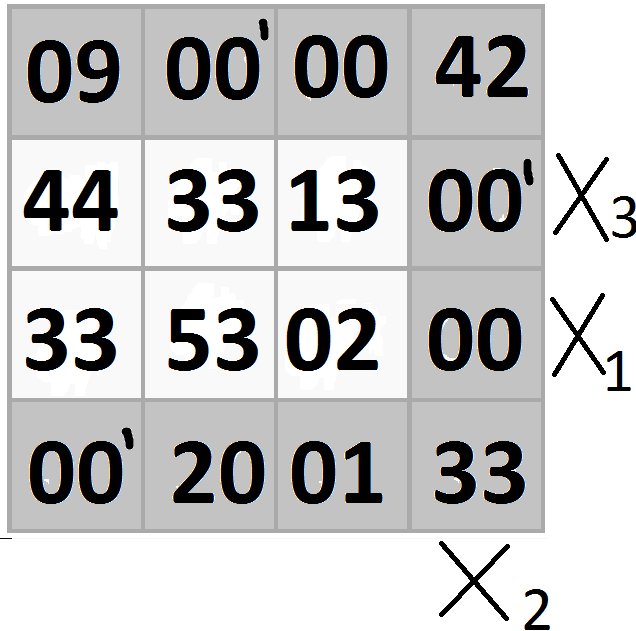
\includegraphics[width=50mm,height=50mm]{select_step_5_Hungarian.png}
	\end{figure}
	
We now end up with the minimum row and column selections we would need to make to select all zeros 
in the graph.  With this we can determine if we are done.  We count our selection lines totalling 
three, as this is less than our set size we move on to step four of the Hungarian Algorithm.  Doing 
this we get fig:[~\ref{fig:select_step_6}] 
	
  	\begin{figure}[H]
		\centering
		\caption{Final State.\label{fig:select_step_6}}
		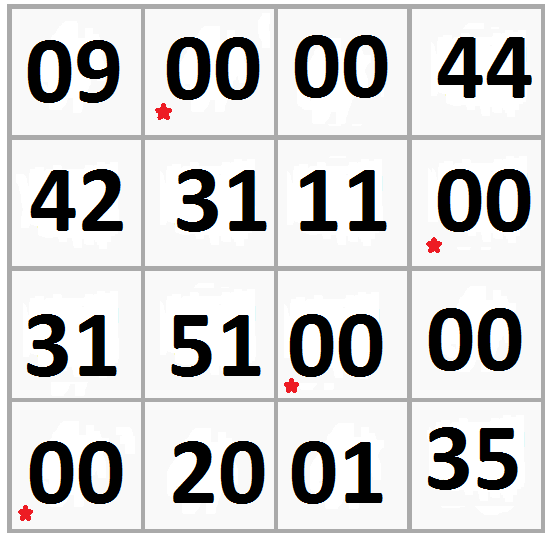
\includegraphics[width=50mm,height=50mm]{select_step_6_Hungarian.png}
	\end{figure}

Now, if necessary, one would rinse and repeat from step 3 to get the minimum cost assignment.  However 
for this example we are now done and get the minimum cost assignment of (row, col)[4,1][1,2][2,4][3,3] 
which going back to fig:[~\ref{fig:select_step_1}] gives a total cost of: 41.  \\

The above is just one way of making the minimum number of selections.  The method was learned from 
wikepedia.

\section{Summary}
This chapter looked into the possibility of using a global optimisation technique for assignment of 
two sets.  We predict that doing so will improve accuracy of the recognition software used by the system.  
We focused on the Hungarian Algorithm as the solution we would implement.  Detailing the steps needed to make it 
work, also noting that eigenfaces method of scoring lends itself nicely to such a minimising solution. \\

Sadly, we cannot in a simple manner implement such a system, as we cannot easily force the Eigenface method to 
provide all the scores of the test data against all training vectors.  There are some hints around the Internet 
as to how to achieve what we wish to do.  For example~\cite{Eigenface_classification} shows us that we could 
extend the \texttt{predict} function to provide us with an array containing the distances scored for each 
training component.  However, it would require diving into OpenCV and extending the existing functionality 
and also could become obsolete if a future superior implementation of the algorithm is designed.  \\

Regardless, time did not permit such alterations to be made within the scope of this work.  Hence this change 
is proposed as possible future work at least until OpenCV provides such functionality itself as was hinted at 
in~\cite{Eigenface_classification}. \\


	
	% conclusionary chapter detailing how i met
	% the "goals" set forth in the Introduction
	\chapter{Conclusion}
	\section{Summing up}
In this work we looked into the viability of creating a facial recognition system with the purpose 
of tracking classroom attendance.  Doing so, we discovered that there are many ways to improve 
recognition rates of such a system both from general normalization methods, as well as ways to use 
the nature of the problem at hand to help in accuracy. \\

The second aspect we noticed was that there was no readily available system that one could test new 
ideas against existing solutions.  At this point, the purpose of this work changed to creating a 
workstation from which a user could add a new normalization technique (or theorised improvement of 
an already existing method) and compare results to past solutions to the targeted problem.  This work
would then use classroom attendance tracking as an accompanying example.

\subsection{Working Example}
As an illustration of the proposed usage of the system this work looked into the viability of the 
Mean Illumination Estimation in conjunction with the Eigenface method of facial recognition both 
in general and specifically for our needs in classroom tracking.  The experiment probed from two 
directions, one; we compared it against OpenCV's inbuilt histogram equalization solution to 
illumination issues.  Two; we ran the experiment twice, one against the Yale B database and again 
against the AT\&T database. \\

The results of this experiment have already been discussed as can be seen in chapter 3.  However, 
a short run-down of the highlights will follow.  MIE works really well when up against strong 
illumination conditions;  directional lighting, strong global change in ambient light etc.  However, 
it greatly degrades the quality of the image worked on meaning it wouldn't work well with  a multiple 
normalisation technique based solution.  \\

It was noted that OpenCV's histogram equalization would suit our classroom environment more adequately 
than MIE as we deal more with global ambient change as opposed to local lighting changes and histogram 
equalization does not have as much of an effect as MIE on the images processed. \\

Nothing done in this work indicates that a system that uses facial recognition to track attendance in a 
classroom environment is an infeasible goal.  We see from the AT\&T database (one that comprises of faces 
taken under similar conditions to what one would expect in a classroom environment) that even before 
normalization techniques are employed, recognition rates are almost within acceptable margins.  Certainly 
no worse than the inaccuracies of the pen and paper approach commonly employed to solve this problem. \\

A more pressing concern would be the total cost of such a system, on that front, this work envisions that such a
system could work with off-the-shelf webcams.  Computationally, most any hardware system would be sufficient as 
computation time would be of little concern.  Indeed (5 - 10) hours could be spent on computation per day and the 
system would still be viable.
 
\subsection{Theory of future work}
Another aspect to this work was to look into the benefits of using a global optimisation technique 
that would replace Eigenface's greedy first match classification system.  This was looked into in depth 
in chapter 4. \\

Due to limitations with the C++ implementation of OpenCV's Eigenface algorithm, such manipulation of its 
inner workings is currently not available to us.  This is not the only project that has wanted a feature 
like this as indicated in the answer to a request for such functionality to be added by the maintainers of OpenCV
~\cite{Eigenface_classification} who replied that they have had many such requests and that it is possible they 
will be adding such functionality at a later stage. \\

Going with this, this work explored how such data could be exploited to yield better accuracies from systems 
where both the training set and test set are known (or should be known).  Having looked specifically at the 
Hungarian algorithm as it offers a solution in polynomial time of O($n^4$)~\cite{munkres1957algorithms}.  Whereas 
any naive solution to the problem (pick all combinations and choose the smallest) would be of O(n!)

\section{Looking ahead}
This work is such that it will never truly be finished, there are many more normalization techniques that 
can be added into the system for comparison, or one could add different recognition algorithms to classify 
test faces.  Examples would include Fisherfaces and Local Binary Patterns Histograms. \\

Strong candidates for future work are solutions to the assignment problem brought up previously  with the 
provided possible solution being the Hungarian algorithm.  Also needed are some form of alignment normalization 
techniques probably something simple to start like using the eyes to align and scale the face.  Both of these 
are pressing issues that will need to be taken into account if one wishes to create an extensive recognition 
system.  \\

Also now that it is clear that such a system can indeed be useful it could be prudent to change over to a C/C++ 
implementation of the working code, this will improve performance in many areas and provide a more in-depth 
control of OpenCV.  \\

If this system is indeed intended for use in classroom attendance tracking then another system will need to 
be devised to compile a set of images per subject and break them up into class sets at the start of each year, 
also allowing for manual addition or removal of students from such a list.


	
	\appendix
	\chapter{Code Extracts}
	These are snippets of code that would have been too large to insert within the main body of the thesis.  What is 
seen below is the implementation of the MIE algorithm (A.1) and (A.2).  When coding the method up I paid little 
attention to efficiency.  \\

Looking at the code snippets we see function d() is our main time sink, (A.1) Lines (12 - 24), and probably the 
area we would want to target when attempting to increase efficiency.  As is, the method is a multiplicative kernel 
of size $11 \times 11$ that needs to be passed over each and every pixel.  \\

As we are dealing with a moving kernel, one optimisation that could be made is instead of complete recalculation 
of the kernel for each pixel, if the kernel moves from left to right, subtract (in our case divide) the elements 
from the left of the kernel and multiply the new right hand elements in (There is a similar case when the kernel 
moves down) doing so we change from $11 \times 11 = 121$ calculations per kernel to $11+11=22$ calculations per 
kernel. \\

The code seen in (A.2) contains the main method for the MIE.  As the algorithm is very mathematically inclined there 
is little here but other function calls.  However, we note specifically the suppression method, (A.1) Lines (53 - 77), which 
encapsulates the core workings of the algorithm passes over each pixel in the image and asks if that pixel should be 
suppressed or highlighted.

\newpage
\begin{lstlisting}[language=Python, caption=MIE Implementation Listing 1\label{Listing:1}]
	def d(x, y, img, n):
		# Mathematically
		# d(x, y) = ln((r(x, y))/(prod{(s,t) E w(nxn)}[ r(s,t) ])^(1/n^2))
		
		prod = long(1);
		kernel_size = n/2;
		kernel_cnt = 0;

		# loop through each element in the kernel multiplying them together.
		# component: prod{(s,t) E w(nxn)}[ r(s,t) ]
		
	# =================================================================== #
		for i in range(-kernel_size + 1, kernel_size, 1):		# y
			for j in range(-kernel_size + 1, kernel_size, 1):	# x
			  # make sure we arnt at centre or going out of bounds of img
				if (((y + i) >= 0) 
						and ((y + i) < len(img)) 
						and ((x + j) >= 0) 
						and ((x+j) < len(img[0]))):
					if (img[y + i][x + j] != 0):
						prod *= long(img[y + i][x + j]);
						kernel_cnt+=1;
	
	# =================================================================== #
	
		denominator = (prod**(1/float(kernel_cnt)));
		if img[y][x] == 0:
			pass;
		temp_in = (img[y][x]) / denominator;
		return math.log(temp_in);
		
	def h(x, y, img, alp, beta, n):
		# Mathematically
		# h(x, y)      = e^[d(x,y)/(alpha*beta)]
		return math.exp( d(x, y, img, n)/ (float(alp) * beta));
		
	def Average_grey(img, n):
		# Mathematically
		# Average_grey = 1/(a*b) Sum{(x,y) E f(axb)}[abs(d(x,y))]
		temp_sum = 0;

		# go through each pixel in image and sum the results of 
		# the d function.
		a, b = len(img), len(img[0]);
		for x in range(0, b, 1):        # x
		   for y in range(0, a, 1):     # y
				temp_d = d(x, y, img, n);
				if (temp_d < 0): temp_d = -temp_d;
				temp_sum += temp_d;

		return (1/(float(len(img)*len(img[0]))) * temp_sum);
		
	# =================================================================== #
	def Supression(img, n, beta):					
		# o_hat(x, y)  = 							    	
		#				{ h(x, y);	h(x, y) <  1	
		#				{ 1;		h(x, y) >= 1	   
		
		sup_img     = np.zeros((len(img), len(img[0])));
		# determine average pixel value							
		gry_ave     = Average_grey(img, n);
		c = 1;
		# go through each pixel and determine if it should be suppressed 
		# or highlighted.
		a, b = len(img), len(img[0]);
		for x in range(0, b, 1):        # x
		   for y in range(0, a, 1):     # y
				Highlight = h(x, y, img, gry_ave, beta, n) # cacl value
				if( Highlight < 1):
					sup_img[y][x]         = Highlight;
					if (Highlight < c): c = Highlight;
				else:
					sup_img[y][x]   = 1;

		return sup_img, c;
		
	# =================================================================== #
\end{lstlisting}

\newpage

\begin{lstlisting}[language=Python, caption = MIE Implementation listing 2\label{Listing:2} ]
	def Mean_Illumination_Estimation_single(img):
		# Implementation of the mean illumination estimation algorithm.
		# takes as input a grey-scaled image and returns the Mean
		# illumination estimation version

		img = convertTo(img, 1);
		# tweak-able values
		# Literature determined that the following value gave best 
		# results for beta.
		beta = 2.2
		
		tmp_f   = (len(img[0])/float(168));
		n = int(tmp_f * 11);  	
							# for testing purposes best set on a per-image  
							# bases via the expression:
							# n 	 = [(width/width_o) * n_o]
							# n_0    = 11
							# width  = curr image face width
							# width_0= database standard width for yale=(168)

		# we first perform the suppression.
		# then build up the solution image by creating a blank slate
		# then determine width and height
		# then build up the new image pixel by pixel
		suppressed, c   = Supression(img, n, beta);
		eqImg           = np.zeros((len(img), len(img[0])), dtype=np.uint8);
		a, b            = len(img), len(img[0]);  
		
		for x in range(0, b, 1):          # x
			for y in range(0, a, 1):	  # y
				# Calc to spread out the highlight values over the spectrum
				tmp = int(((255*(suppressed[y][x] - c))/(1-c)));
				eqImg[y][x] = tmp;

		return eqImg;
\end{lstlisting}


	
	% =================== =================== %
	\addcontentsline{toc}{chapter}{References} 
	\bibliographystyle{rucsacm}
	\bibliography{thesis}
\end{document}
